% Options for packages loaded elsewhere
\PassOptionsToPackage{unicode}{hyperref}
\PassOptionsToPackage{hyphens}{url}
%
\documentclass[
]{article}
\usepackage{lmodern}
\usepackage{amssymb,amsmath}
\usepackage{ifxetex,ifluatex}
\ifnum 0\ifxetex 1\fi\ifluatex 1\fi=0 % if pdftex
  \usepackage[T1]{fontenc}
  \usepackage[utf8]{inputenc}
  \usepackage{textcomp} % provide euro and other symbols
\else % if luatex or xetex
  \usepackage{unicode-math}
  \defaultfontfeatures{Scale=MatchLowercase}
  \defaultfontfeatures[\rmfamily]{Ligatures=TeX,Scale=1}
\fi
% Use upquote if available, for straight quotes in verbatim environments
\IfFileExists{upquote.sty}{\usepackage{upquote}}{}
\IfFileExists{microtype.sty}{% use microtype if available
  \usepackage[]{microtype}
  \UseMicrotypeSet[protrusion]{basicmath} % disable protrusion for tt fonts
}{}
\makeatletter
\@ifundefined{KOMAClassName}{% if non-KOMA class
  \IfFileExists{parskip.sty}{%
    \usepackage{parskip}
  }{% else
    \setlength{\parindent}{0pt}
    \setlength{\parskip}{6pt plus 2pt minus 1pt}}
}{% if KOMA class
  \KOMAoptions{parskip=half}}
\makeatother
\usepackage{xcolor}
\IfFileExists{xurl.sty}{\usepackage{xurl}}{} % add URL line breaks if available
\IfFileExists{bookmark.sty}{\usepackage{bookmark}}{\usepackage{hyperref}}
\hypersetup{
  hidelinks,
  pdfcreator={LaTeX via pandoc}}
\urlstyle{same} % disable monospaced font for URLs
\usepackage[margin=1in]{geometry}
\usepackage{color}
\usepackage{fancyvrb}
\newcommand{\VerbBar}{|}
\newcommand{\VERB}{\Verb[commandchars=\\\{\}]}
\DefineVerbatimEnvironment{Highlighting}{Verbatim}{commandchars=\\\{\}}
% Add ',fontsize=\small' for more characters per line
\usepackage{framed}
\definecolor{shadecolor}{RGB}{48,48,48}
\newenvironment{Shaded}{\begin{snugshade}}{\end{snugshade}}
\newcommand{\AlertTok}[1]{\textcolor[rgb]{1.00,0.81,0.69}{#1}}
\newcommand{\AnnotationTok}[1]{\textcolor[rgb]{0.50,0.62,0.50}{\textbf{#1}}}
\newcommand{\AttributeTok}[1]{\textcolor[rgb]{0.80,0.80,0.80}{#1}}
\newcommand{\BaseNTok}[1]{\textcolor[rgb]{0.86,0.64,0.64}{#1}}
\newcommand{\BuiltInTok}[1]{\textcolor[rgb]{0.80,0.80,0.80}{#1}}
\newcommand{\CharTok}[1]{\textcolor[rgb]{0.86,0.64,0.64}{#1}}
\newcommand{\CommentTok}[1]{\textcolor[rgb]{0.50,0.62,0.50}{#1}}
\newcommand{\CommentVarTok}[1]{\textcolor[rgb]{0.50,0.62,0.50}{\textbf{#1}}}
\newcommand{\ConstantTok}[1]{\textcolor[rgb]{0.86,0.64,0.64}{\textbf{#1}}}
\newcommand{\ControlFlowTok}[1]{\textcolor[rgb]{0.94,0.87,0.69}{#1}}
\newcommand{\DataTypeTok}[1]{\textcolor[rgb]{0.87,0.87,0.75}{#1}}
\newcommand{\DecValTok}[1]{\textcolor[rgb]{0.86,0.86,0.80}{#1}}
\newcommand{\DocumentationTok}[1]{\textcolor[rgb]{0.50,0.62,0.50}{#1}}
\newcommand{\ErrorTok}[1]{\textcolor[rgb]{0.76,0.75,0.62}{#1}}
\newcommand{\ExtensionTok}[1]{\textcolor[rgb]{0.80,0.80,0.80}{#1}}
\newcommand{\FloatTok}[1]{\textcolor[rgb]{0.75,0.75,0.82}{#1}}
\newcommand{\FunctionTok}[1]{\textcolor[rgb]{0.94,0.94,0.56}{#1}}
\newcommand{\ImportTok}[1]{\textcolor[rgb]{0.80,0.80,0.80}{#1}}
\newcommand{\InformationTok}[1]{\textcolor[rgb]{0.50,0.62,0.50}{\textbf{#1}}}
\newcommand{\KeywordTok}[1]{\textcolor[rgb]{0.94,0.87,0.69}{#1}}
\newcommand{\NormalTok}[1]{\textcolor[rgb]{0.80,0.80,0.80}{#1}}
\newcommand{\OperatorTok}[1]{\textcolor[rgb]{0.94,0.94,0.82}{#1}}
\newcommand{\OtherTok}[1]{\textcolor[rgb]{0.94,0.94,0.56}{#1}}
\newcommand{\PreprocessorTok}[1]{\textcolor[rgb]{1.00,0.81,0.69}{\textbf{#1}}}
\newcommand{\RegionMarkerTok}[1]{\textcolor[rgb]{0.80,0.80,0.80}{#1}}
\newcommand{\SpecialCharTok}[1]{\textcolor[rgb]{0.86,0.64,0.64}{#1}}
\newcommand{\SpecialStringTok}[1]{\textcolor[rgb]{0.80,0.58,0.58}{#1}}
\newcommand{\StringTok}[1]{\textcolor[rgb]{0.80,0.58,0.58}{#1}}
\newcommand{\VariableTok}[1]{\textcolor[rgb]{0.80,0.80,0.80}{#1}}
\newcommand{\VerbatimStringTok}[1]{\textcolor[rgb]{0.80,0.58,0.58}{#1}}
\newcommand{\WarningTok}[1]{\textcolor[rgb]{0.50,0.62,0.50}{\textbf{#1}}}
\usepackage{graphicx}
\makeatletter
\def\maxwidth{\ifdim\Gin@nat@width>\linewidth\linewidth\else\Gin@nat@width\fi}
\def\maxheight{\ifdim\Gin@nat@height>\textheight\textheight\else\Gin@nat@height\fi}
\makeatother
% Scale images if necessary, so that they will not overflow the page
% margins by default, and it is still possible to overwrite the defaults
% using explicit options in \includegraphics[width, height, ...]{}
\setkeys{Gin}{width=\maxwidth,height=\maxheight,keepaspectratio}
% Set default figure placement to htbp
\makeatletter
\def\fps@figure{htbp}
\makeatother
\setlength{\emergencystretch}{3em} % prevent overfull lines
\providecommand{\tightlist}{%
  \setlength{\itemsep}{0pt}\setlength{\parskip}{0pt}}
\setcounter{secnumdepth}{-\maxdimen} % remove section numbering

\title{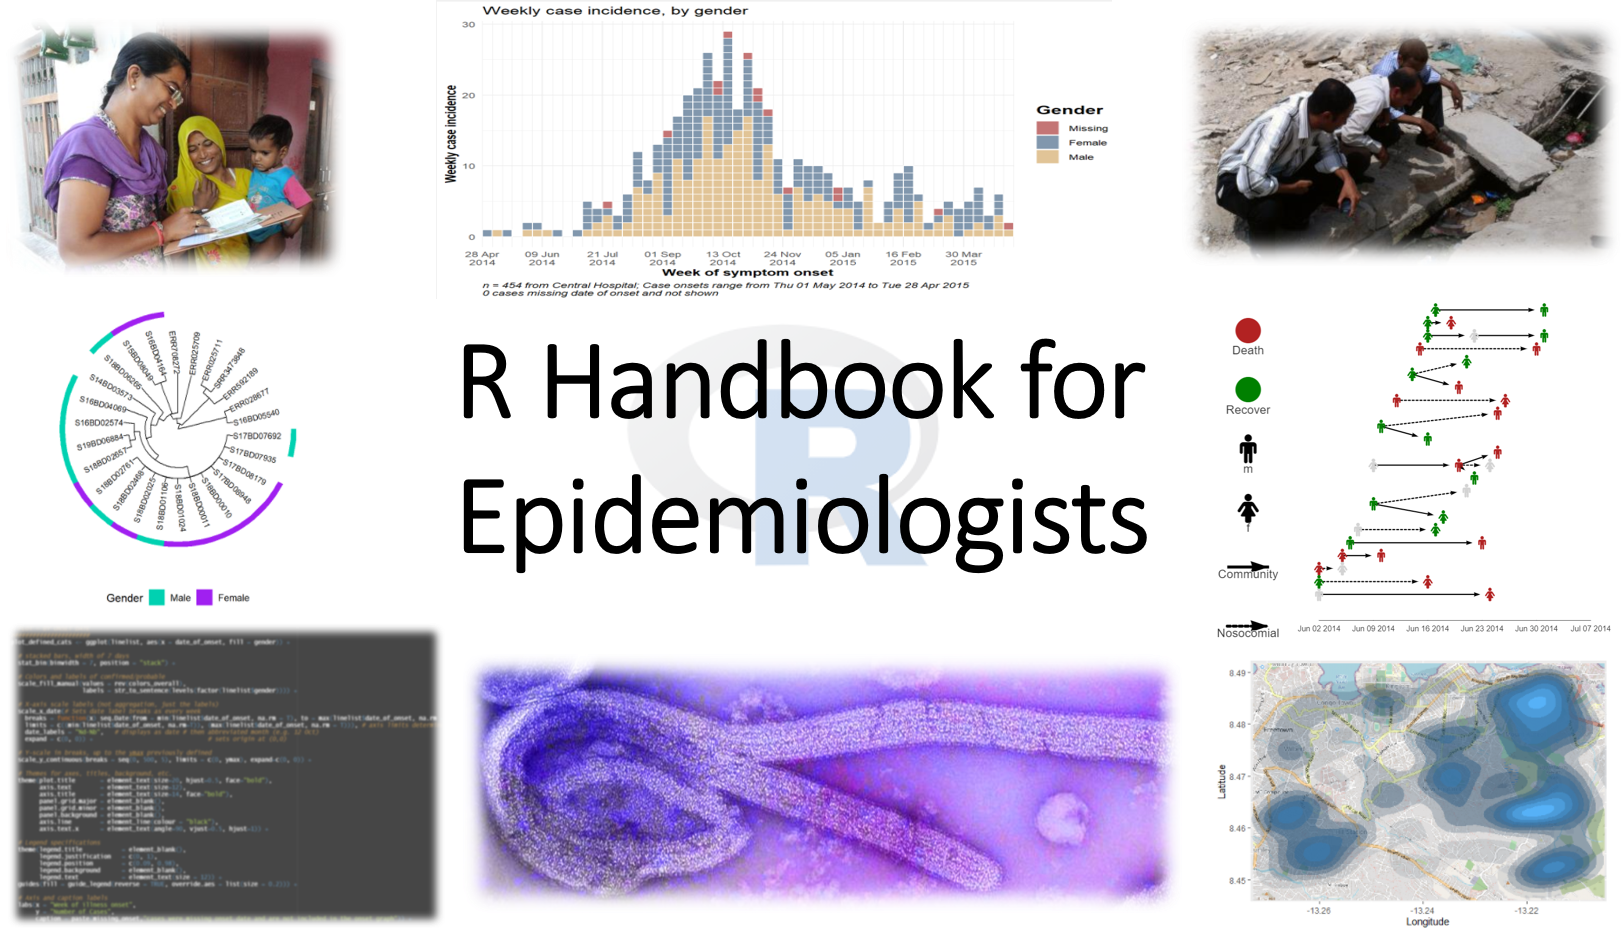
\includegraphics{../images/R Handbook Logo.png}}
\author{}
\date{\vspace{-2.5em}Produced Sunday 27 December 2020}

\begin{document}
\maketitle

{
\setcounter{tocdepth}{3}
\tableofcontents
}
\textbf{This is one page of the R Handbook for Epidemiologists, but is
being printed as a stand-alone page.}

\textbf{You can find the complete handbook on
\href{https://github.com/nsbatra/Epi_R_handbook}{Github}}

\hypertarget{age_pyramid}{%
\section{Age Pyramids}\label{age_pyramid}}

Age pyramids can be useful to show patterns by age group. They can show
gender, or the distribution of other characteristics.\\
These tabs demonstrate how to produce age pyramids using:

\begin{itemize}
\tightlist
\item
  Fast \& easy: Using the \textbf{apyramid} package\\
\item
  More flexible: Using \texttt{ggplot()}\\
\item
  Having baseline demographics displayed in the background of the
  pyramid\\
\item
  Using pyramid-style plots to show other types of data (e.g responses
  to Likert-style questions)
\end{itemize}

\hypertarget{overview}{%
\subsection{Overview}\label{overview}}

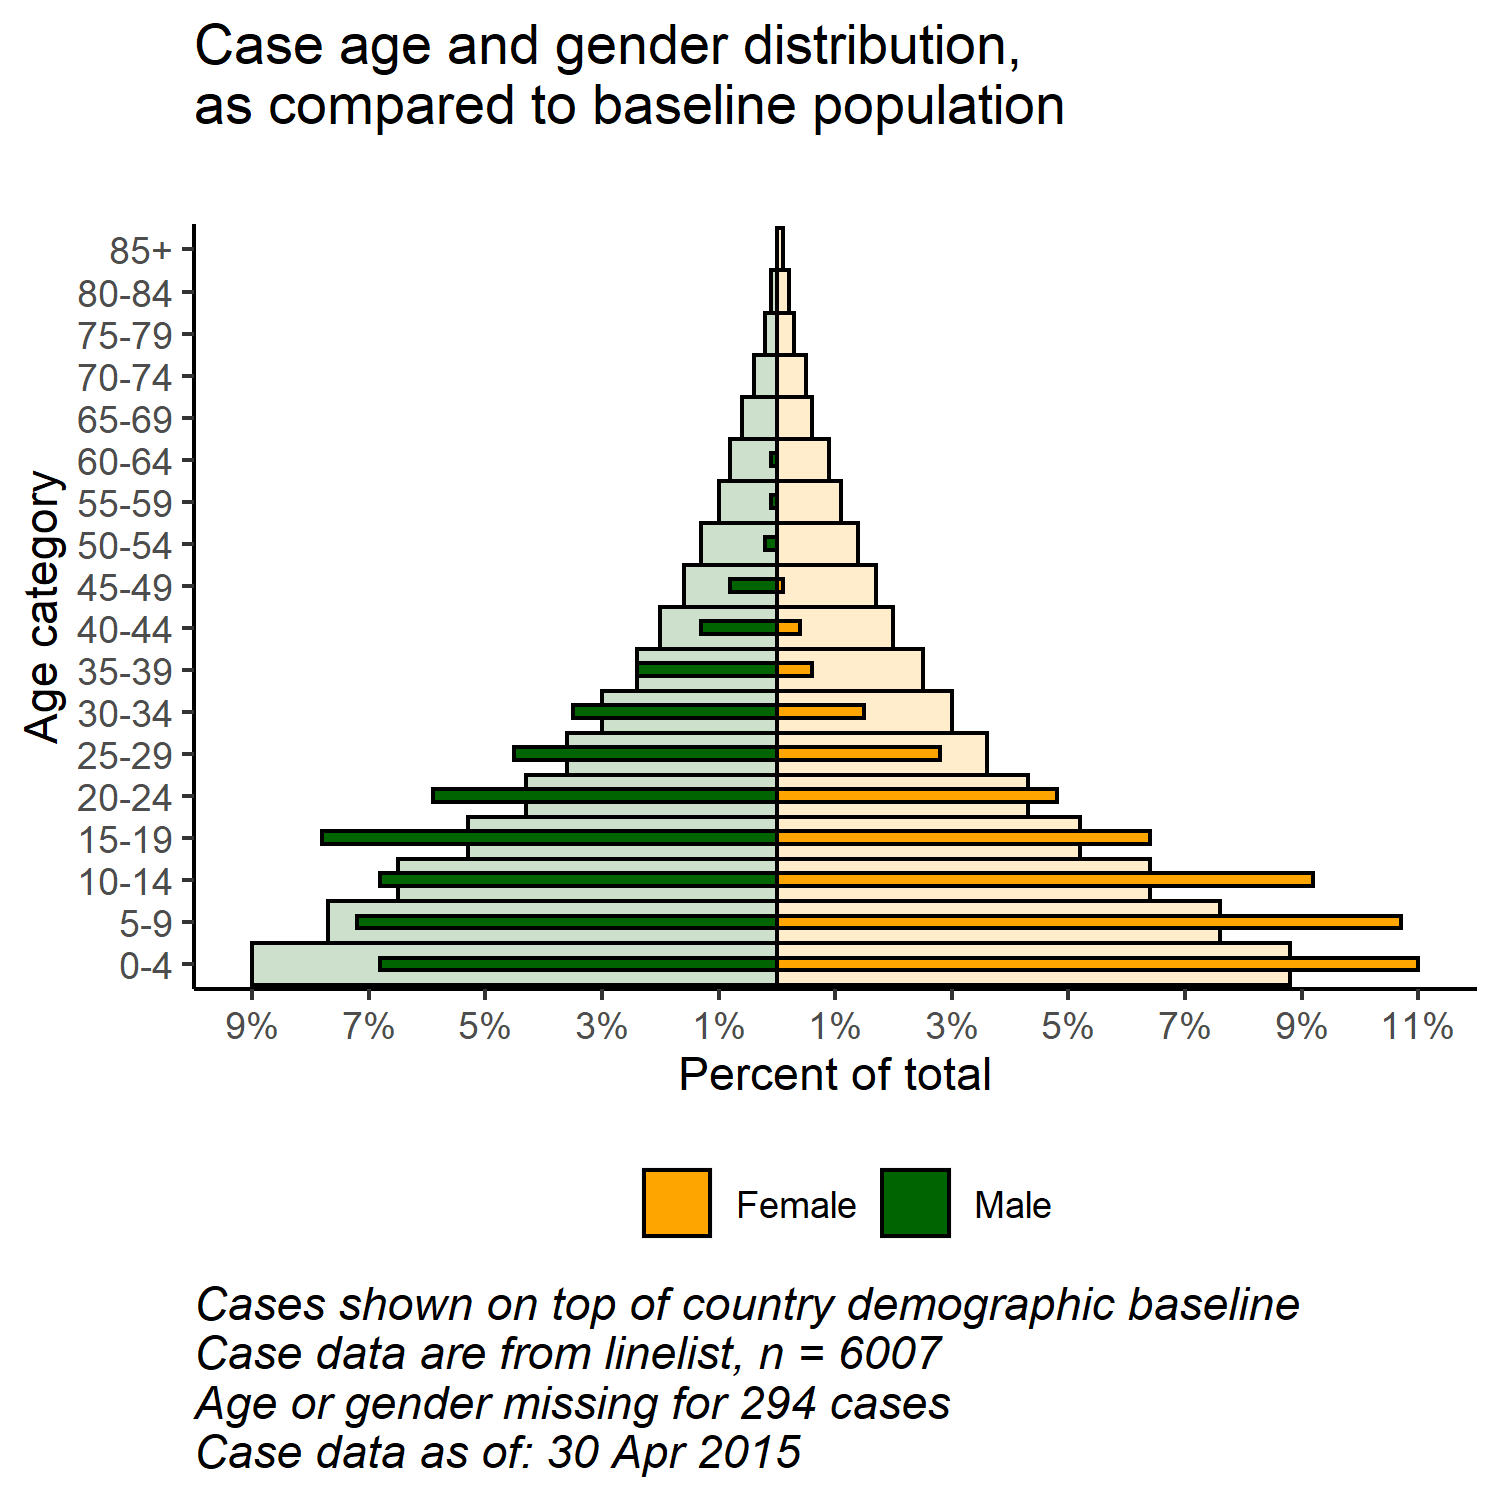
\includegraphics[width=0.5\linewidth]{C:/Users/Neale/OneDrive - Neale Batra/Documents/Analytic Software/R/Projects/R handbook/Epi_R_handbook/images/pop_pyramid_baseline}
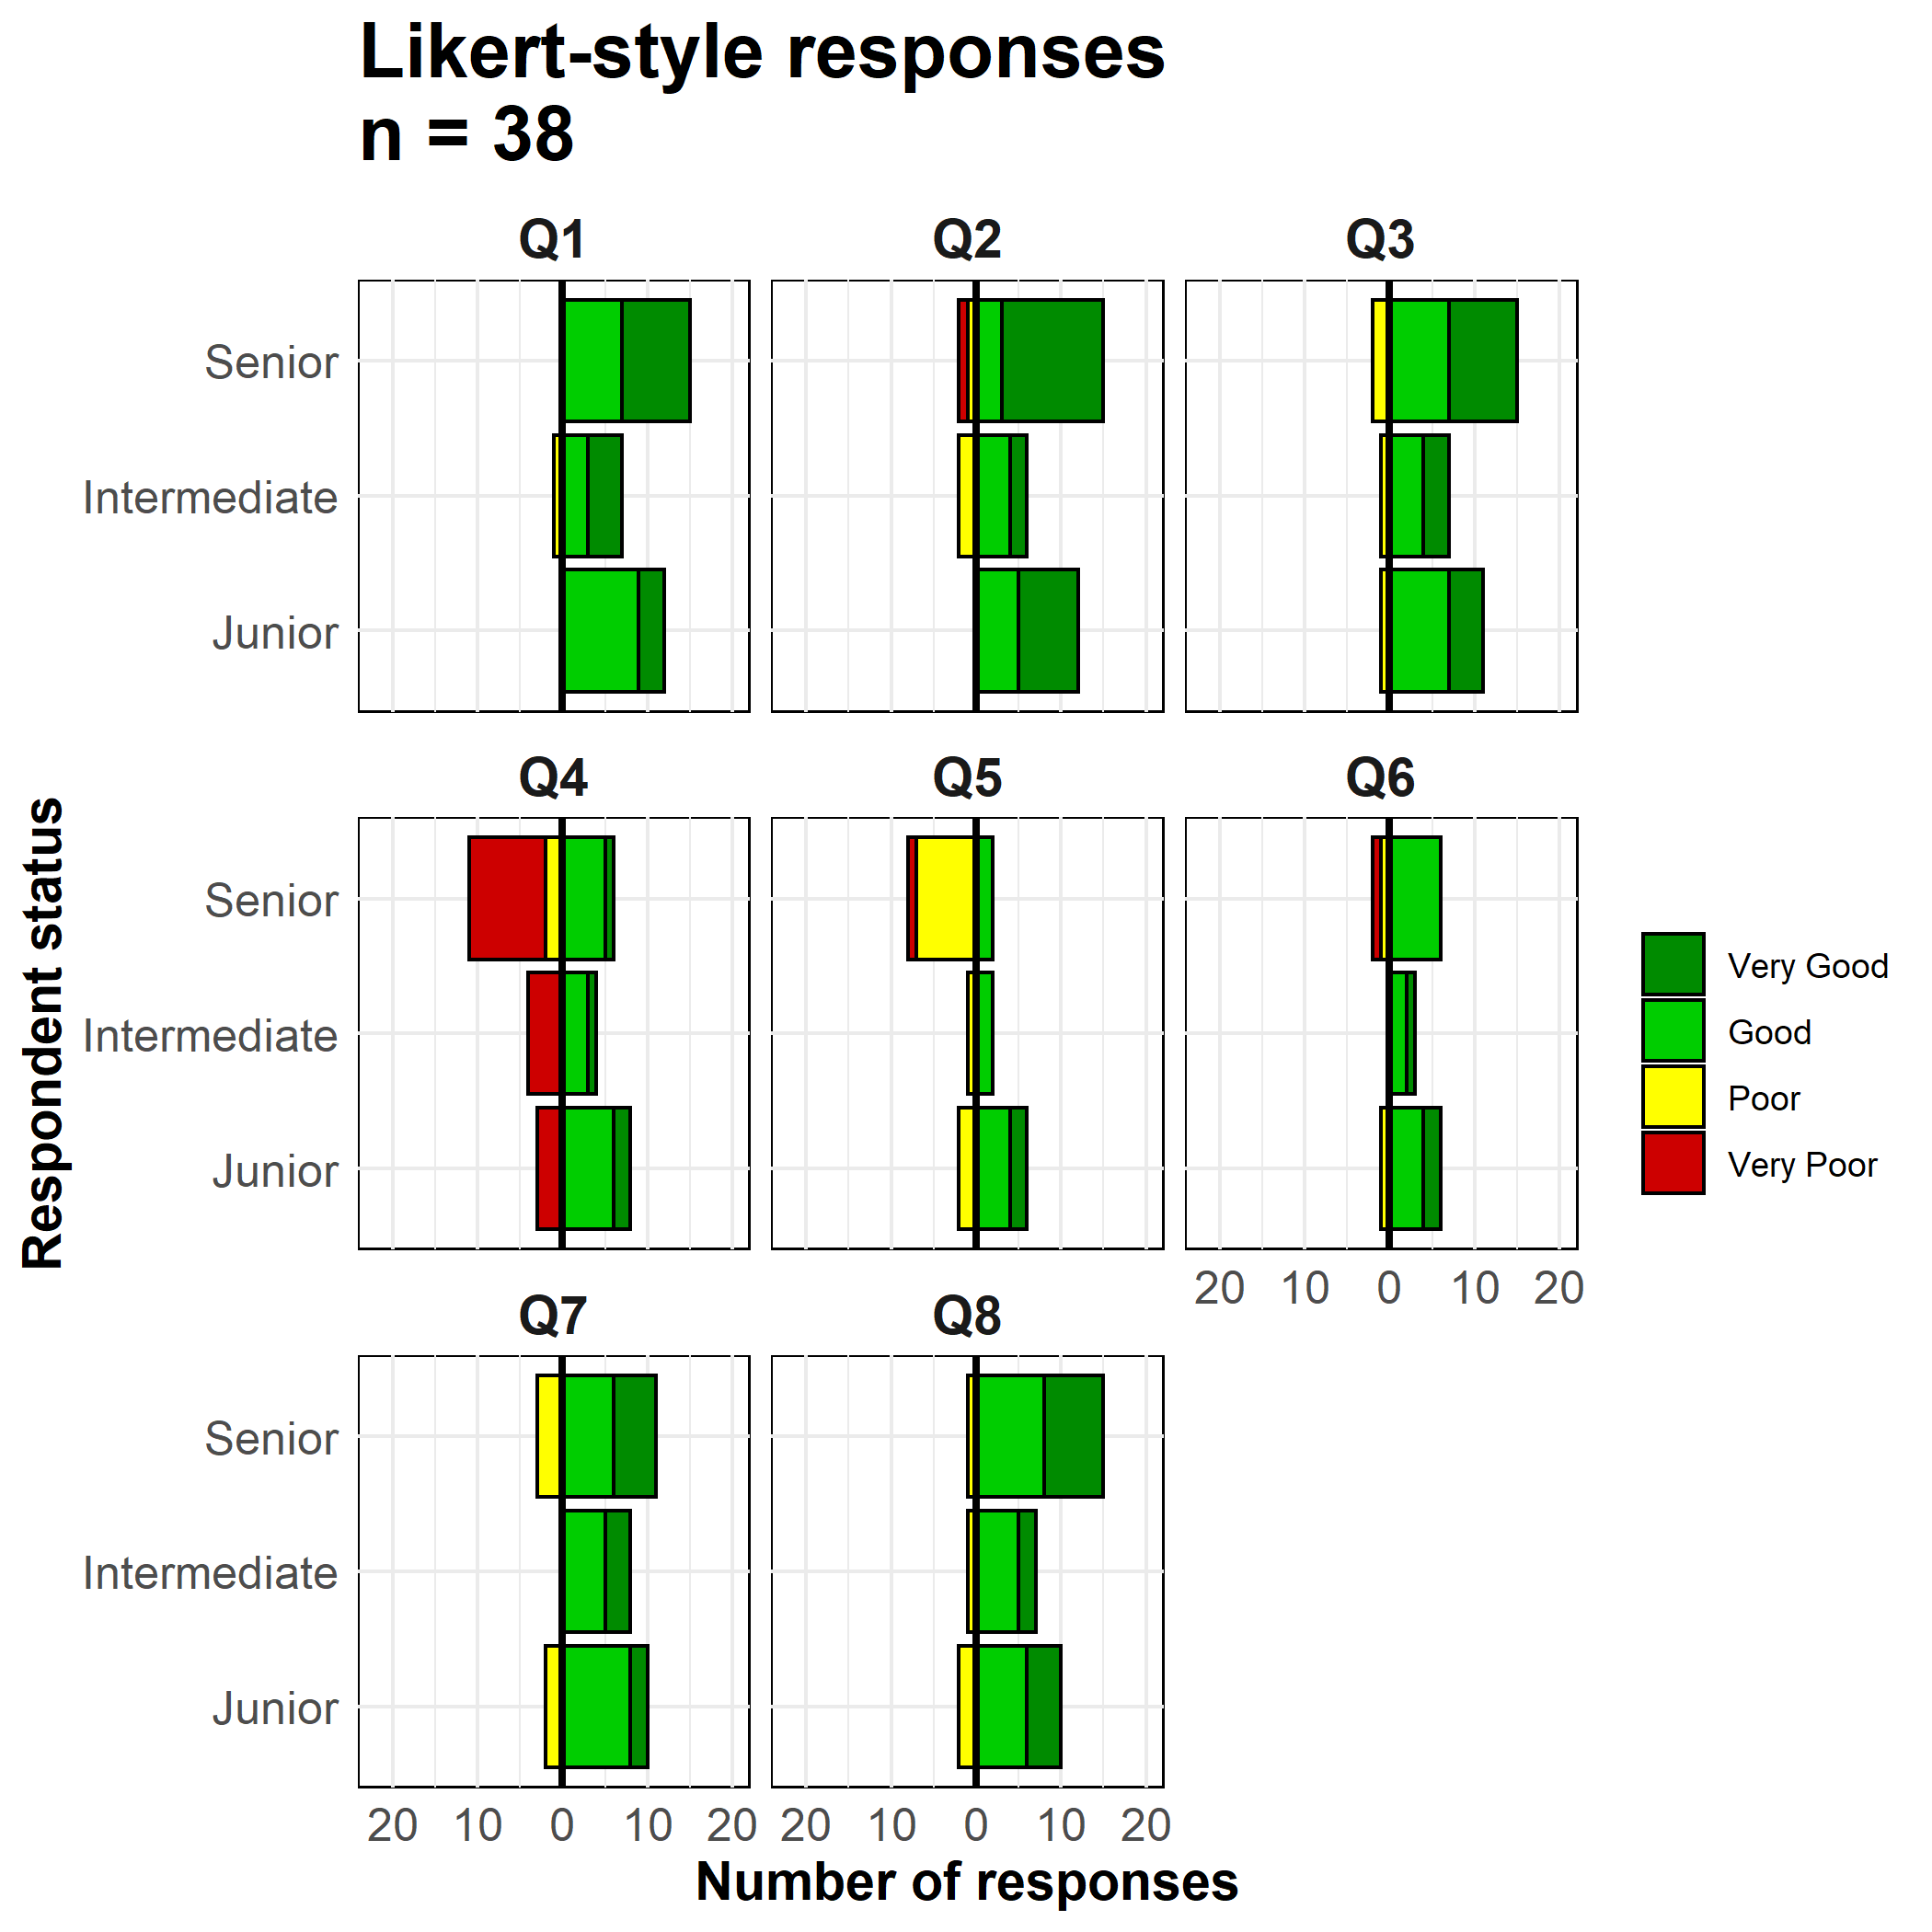
\includegraphics[width=0.5\linewidth]{C:/Users/Neale/OneDrive - Neale Batra/Documents/Analytic Software/R/Projects/R handbook/Epi_R_handbook/images/likert}

Age/gender demographic pyramids in R are generally made with
\texttt{ggplot()} by creating two barplots (one for each gender),
converting one's values to negative values, and flipping the x and y
axes to display the barplots vertically.

Here we offer a quick approach through the \textbf{apyramid} package:

\begin{itemize}
\tightlist
\item
  More customizable code using the raw \texttt{ggplot()} commands\\
\item
  How to combine case demographic data and compare with that of a
  baseline population (as shown above)\\
\item
  Application of these methods to show other types of data
  (e.g.~responses to Likert-style survey questions)
\end{itemize}

\hypertarget{preparation}{%
\subsection{Preparation}\label{preparation}}

For this tab we use the \texttt{linelist} dataset that is cleaned in the
Cleaning tab.

To make a traditional age/sex demographic pyramid, the data must first
be cleaned in the following ways:

\begin{itemize}
\tightlist
\item
  The gender column must be cleaned.\\
\item
  Age should be in an age category column, and should be an of class
  Factor (with correctly ordered levels)
\end{itemize}

\textbf{Load packages}

First, load the packages required for this analysis:

\begin{Shaded}
\begin{Highlighting}[]
\NormalTok{pacman}\OperatorTok{::}\KeywordTok{p\_load}\NormalTok{(rio,       }\CommentTok{\# to import data}
\NormalTok{               here,      }\CommentTok{\# to locate files}
\NormalTok{               tidyverse, }\CommentTok{\# to clean, handle, and plot the data (includes ggplot2 package)}
\NormalTok{               apyramid,  }\CommentTok{\# a package dedicated to creating age pyramids}
\NormalTok{               stringr)   }\CommentTok{\# working with strings for titles, captions, etc.}
\end{Highlighting}
\end{Shaded}

Load the data

\begin{Shaded}
\begin{Highlighting}[]
\NormalTok{linelist \textless{}{-}}\StringTok{ }\NormalTok{rio}\OperatorTok{::}\KeywordTok{import}\NormalTok{(}\StringTok{"linelist\_cleaned.csv"}\NormalTok{)}
\end{Highlighting}
\end{Shaded}

\textbf{Check class of variables}

Ensure that the age variable is class Numeric, and check the class and
order of levels of \texttt{age\_cat} and \texttt{age\_cat5}

\begin{Shaded}
\begin{Highlighting}[]
\KeywordTok{class}\NormalTok{(linelist}\OperatorTok{$}\NormalTok{age\_years)}
\CommentTok{\#\# [1] "numeric"}

\KeywordTok{class}\NormalTok{(linelist}\OperatorTok{$}\NormalTok{age\_cat)}
\CommentTok{\#\# [1] "factor"}
\KeywordTok{class}\NormalTok{(linelist}\OperatorTok{$}\NormalTok{age\_cat5)}
\CommentTok{\#\# [1] "factor"}

\KeywordTok{table}\NormalTok{(linelist}\OperatorTok{$}\NormalTok{age\_cat, }\DataTypeTok{useNA =} \StringTok{"always"}\NormalTok{)}
\CommentTok{\#\# }
\CommentTok{\#\#   0{-}4   5{-}9 10{-}14 15{-}19 20{-}29 30{-}49 50{-}69   70+  \textless{}NA\textgreater{} }
\CommentTok{\#\#  1172  1130   995   895  1090   605    26     0    92}
\KeywordTok{table}\NormalTok{(linelist}\OperatorTok{$}\NormalTok{age\_cat5, }\DataTypeTok{useNA =} \StringTok{"always"}\NormalTok{)}
\CommentTok{\#\# }
\CommentTok{\#\#   0{-}4   5{-}9 10{-}14 15{-}19 20{-}24 25{-}29 30{-}34 35{-}39 40{-}44 45{-}49 50{-}54 55{-}59 60{-}64 }
\CommentTok{\#\#  1172  1130   995   895   649   441   294   179    86    46    21     4     1 }
\CommentTok{\#\# 65{-}69 70{-}74 75{-}79 80{-}84   85+  \textless{}NA\textgreater{} }
\CommentTok{\#\#     0     0     0     0     0    92}
\end{Highlighting}
\end{Shaded}

\hypertarget{apyramid-package}{%
\subsection{\texorpdfstring{\textbf{apyramid}
package}{apyramid package}}\label{apyramid-package}}

The package \textbf{apyramid} allows you to quickly make an age pyramid.
For more nuanced situations, see the tab on using \texttt{ggplot()} to
make age pyramids. You can read more about the \textbf{apyramid} package
in its Help page by entering \texttt{?age\_pyramid} in your R console.

\hypertarget{age_pyramid-with-linelist-data}{%
\subsubsection{\texorpdfstring{\texttt{age\_pyramid()} with linelist
data}{age\_pyramid() with linelist data}}\label{age_pyramid-with-linelist-data}}

Using the cleaned linelist dataset, we can create an age pyramid with
just one simple command. If you need help cleaning your data, see the
handbook page on Cleaning data (LINK). In this command:

\begin{itemize}
\tightlist
\item
  The \emph{data} argument is set as the \texttt{linelist} dataframe\\
\item
  The \emph{age\_group} argument is set to the name (in quotes) of the
  numeric category variable (in this case \texttt{age\_cat5})\\
\item
  The \emph{split\_by} argument (bar colors) should be a binary column
  (in this case ``gender'')
\end{itemize}

\begin{Shaded}
\begin{Highlighting}[]
\NormalTok{apyramid}\OperatorTok{::}\KeywordTok{age\_pyramid}\NormalTok{(}\DataTypeTok{data =}\NormalTok{ linelist,}
                      \DataTypeTok{age\_group =} \StringTok{"age\_cat5"}\NormalTok{,}
                      \DataTypeTok{split\_by =} \StringTok{"gender"}\NormalTok{)}
\end{Highlighting}
\end{Shaded}

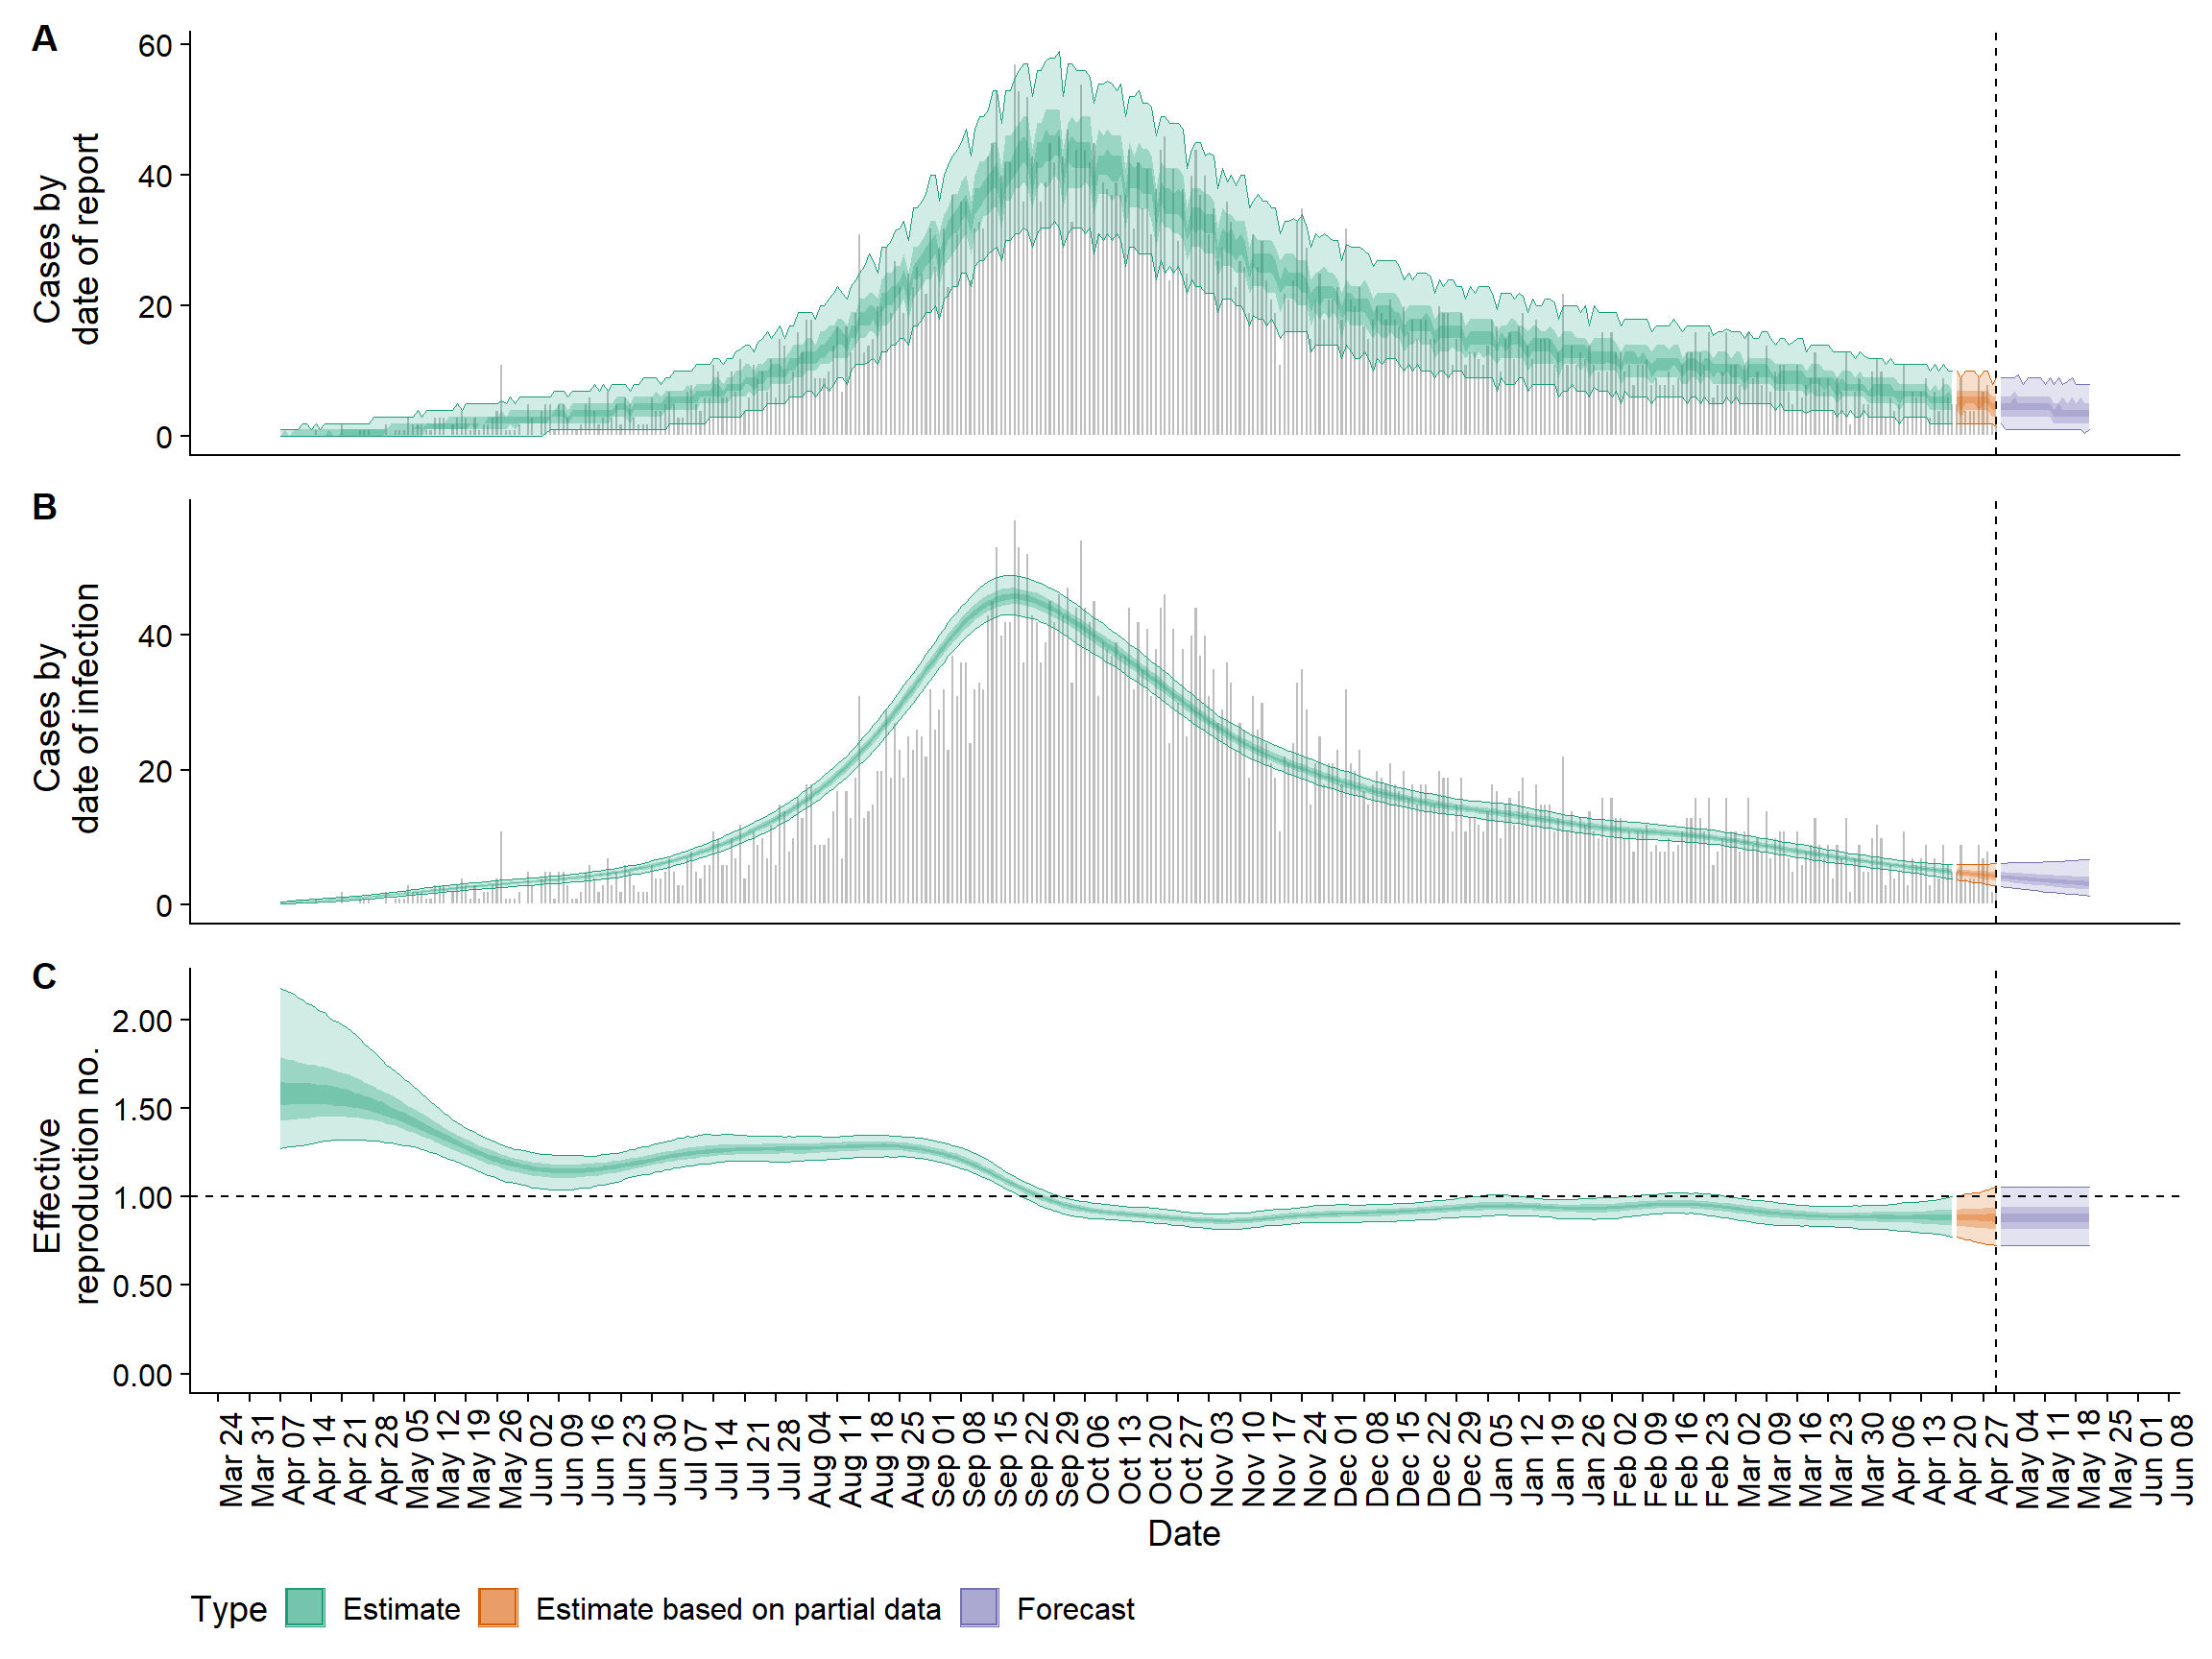
\includegraphics{C:/Users/Neale/ONEDRI~1/DOCUME~1/ANALYT~1/R/Projects/RHANDB~1/EPI_R_~1/pages_OUTPU~1/AGE_PY~1/figure-latex/unnamed-chunk-7-1.pdf}
When using \textbf{agepyramid} package, if the \texttt{split\_by} column
is binary (e.g.~male/female, or yes/no), then the result will appear as
a pyramid. However if there are more than two values in the
\texttt{split\_by} column (not including \texttt{NA}), the pyramid will
appears as a faceted barplot with empty bars in the background
indicating the range of the un-faceted data set for the age group.
Values of split\_by will appear as labels at top of each facet. For
example below if the \texttt{split\_by} variable is ``hospital''.

\begin{Shaded}
\begin{Highlighting}[]
\NormalTok{apyramid}\OperatorTok{::}\KeywordTok{age\_pyramid}\NormalTok{(}\DataTypeTok{data =}\NormalTok{ linelist,}
                      \DataTypeTok{age\_group =} \StringTok{"age\_cat5"}\NormalTok{,}
                      \DataTypeTok{split\_by =} \StringTok{"hospital"}\NormalTok{,}
                      \DataTypeTok{na.rm =} \OtherTok{FALSE}\NormalTok{)        }\CommentTok{\# show a bar for patients missing age, (note: this changes the pyramid into a faceted barplot)}
\end{Highlighting}
\end{Shaded}

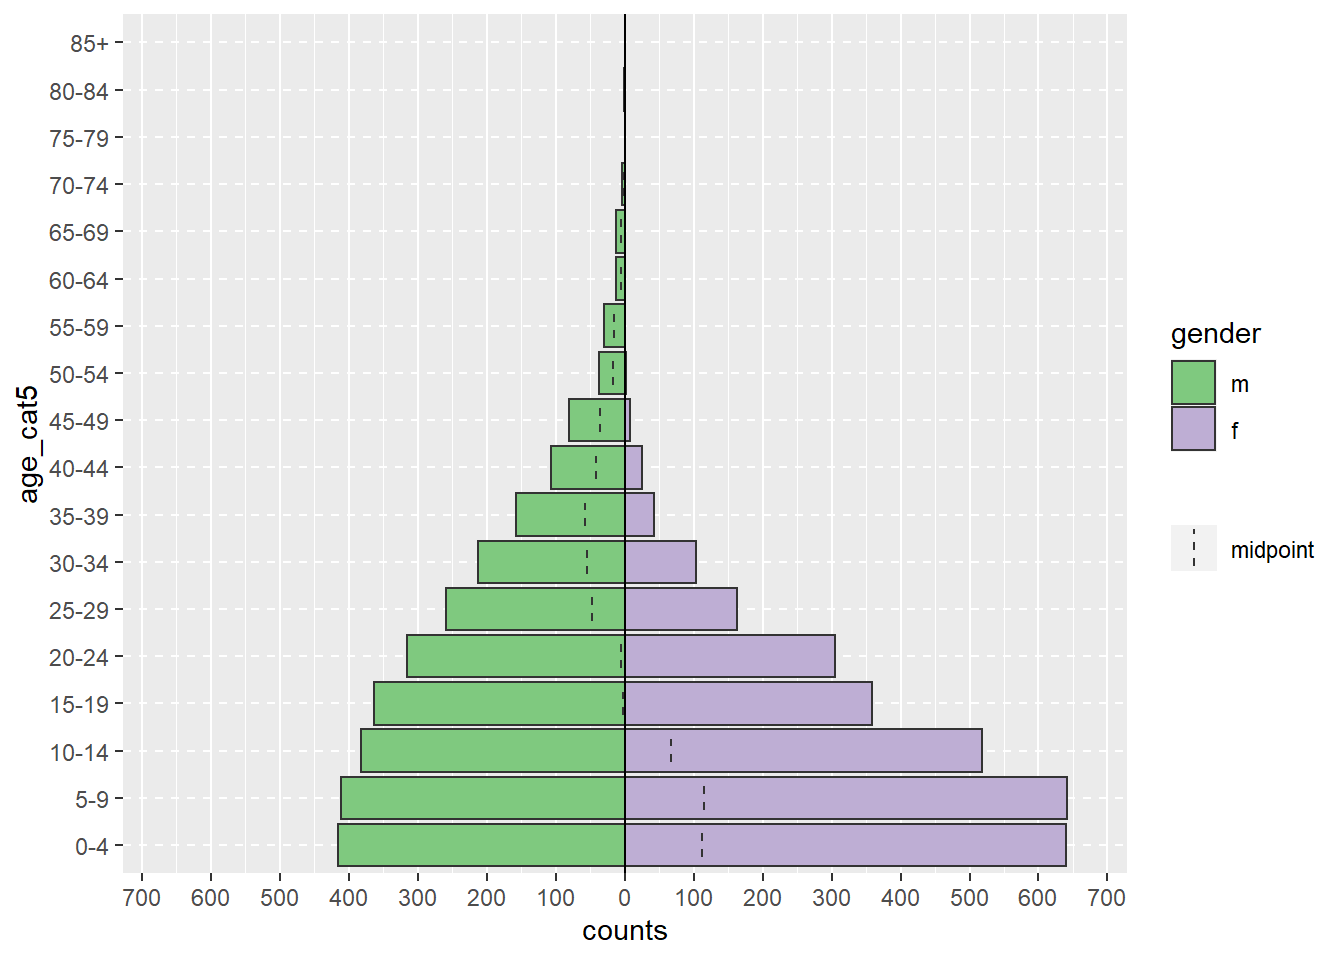
\includegraphics{C:/Users/Neale/ONEDRI~1/DOCUME~1/ANALYT~1/R/Projects/RHANDB~1/EPI_R_~1/pages_OUTPU~1/AGE_PY~1/figure-latex/unnamed-chunk-8-1.pdf}

\textbf{Missing values}\\
Rows missing values for the \texttt{split\_by} or \texttt{age\_group}
columns, if coded as \texttt{NA}, will not trigger the faceting shown
above. By default these rows will not be shown. However you can specify
that they appear, in an adjacent barplot and as a separate age group at
the top, by specifying \texttt{na.rm\ =\ FALSE}.

\begin{Shaded}
\begin{Highlighting}[]
\NormalTok{apyramid}\OperatorTok{::}\KeywordTok{age\_pyramid}\NormalTok{(}\DataTypeTok{data =}\NormalTok{ linelist,}
                      \DataTypeTok{age\_group =} \StringTok{"age\_cat5"}\NormalTok{,}
                      \DataTypeTok{split\_by =} \StringTok{"gender"}\NormalTok{,}
                      \DataTypeTok{na.rm =} \OtherTok{FALSE}\NormalTok{)         }\CommentTok{\# show patients missing age or gender}
\end{Highlighting}
\end{Shaded}

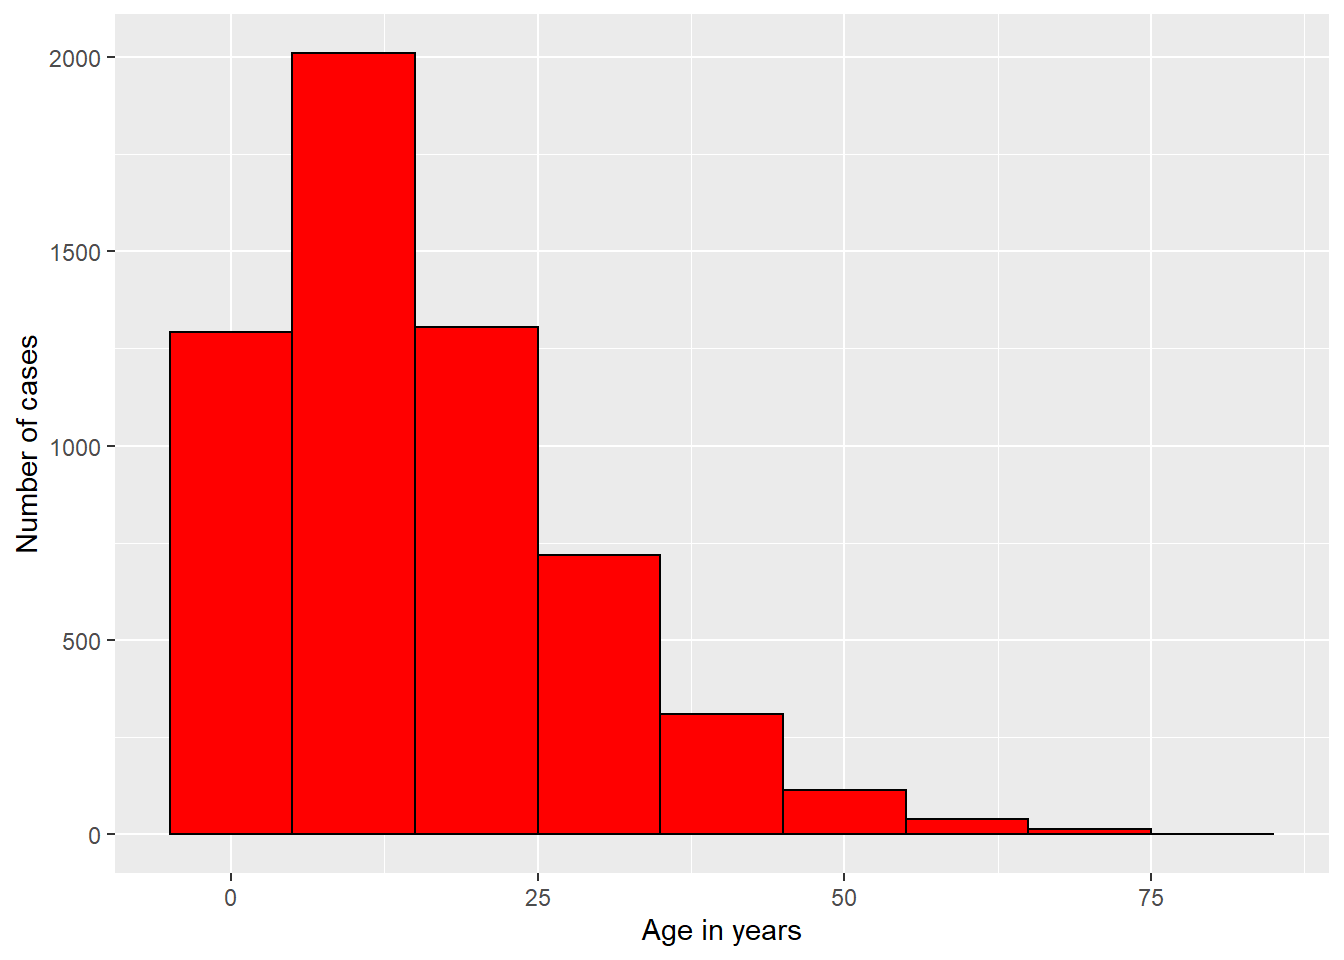
\includegraphics{C:/Users/Neale/ONEDRI~1/DOCUME~1/ANALYT~1/R/Projects/RHANDB~1/EPI_R_~1/pages_OUTPU~1/AGE_PY~1/figure-latex/unnamed-chunk-9-1.pdf}

\textbf{Proportions, colors, \& aesthetics}

By default, the bars display counts (not \%), a dashed mid-line for each
group is shown, and the colors are green/purple. Each of these
parameters can all be adjusted, as shown below:

You can also add additional \texttt{ggplot()} commands to the plot using
the standard \texttt{ggplot()} ``+'' syntax, such as aesthetic themes
and label adjustments:

\begin{Shaded}
\begin{Highlighting}[]
\NormalTok{apyramid}\OperatorTok{::}\KeywordTok{age\_pyramid}\NormalTok{(}\DataTypeTok{data =}\NormalTok{ linelist,}
                      \DataTypeTok{age\_group =} \StringTok{"age\_cat5"}\NormalTok{,}
                      \DataTypeTok{split\_by =} \StringTok{"gender"}\NormalTok{,}
                      \DataTypeTok{proportional =} \OtherTok{TRUE}\NormalTok{,                  }\CommentTok{\# show percents, not counts}
                      \DataTypeTok{show\_midpoint =} \OtherTok{FALSE}\NormalTok{,                }\CommentTok{\# remove bar mid{-}point line}
                      \CommentTok{\#pal = c("orange", "purple")          \# can specify alt. colors here (but not labels, see below)}
\NormalTok{                      )}\OperatorTok{+}\StringTok{                 }
\StringTok{  }
\StringTok{  }\CommentTok{\# additional ggplot commands}
\StringTok{  }\KeywordTok{theme\_minimal}\NormalTok{()}\OperatorTok{+}\StringTok{                                          }\CommentTok{\# simplify the background}
\StringTok{  }\KeywordTok{scale\_fill\_manual}\NormalTok{(}\DataTypeTok{values =} \KeywordTok{c}\NormalTok{(}\StringTok{"orange"}\NormalTok{, }\StringTok{"purple"}\NormalTok{),         }\CommentTok{\# to specify colors AND labels}
                     \DataTypeTok{labels =} \KeywordTok{c}\NormalTok{(}\StringTok{"Male"}\NormalTok{, }\StringTok{"Female"}\NormalTok{))}\OperatorTok{+}
\StringTok{  }\KeywordTok{labs}\NormalTok{(}\DataTypeTok{y =} \StringTok{"Percent of all cases"}\NormalTok{,                          }\CommentTok{\# note that x and y labels are switched (see ggplot tab)}
       \DataTypeTok{x =} \StringTok{"Age categories"}\NormalTok{,                          }
       \DataTypeTok{fill =} \StringTok{"Gender"}\NormalTok{, }
       \DataTypeTok{caption =} \StringTok{"My data source and caption here"}\NormalTok{,}
       \DataTypeTok{title =} \StringTok{"Title of my plot"}\NormalTok{,}
       \DataTypeTok{subtitle =} \StringTok{"Subtitle with }\CharTok{\textbackslash{}n}\StringTok{ a second line..."}\NormalTok{)}\OperatorTok{+}
\StringTok{  }\KeywordTok{theme}\NormalTok{(}
    \DataTypeTok{legend.position =} \StringTok{"bottom"}\NormalTok{,                             }\CommentTok{\# move legend to bottom}
    \DataTypeTok{axis.text =} \KeywordTok{element\_text}\NormalTok{(}\DataTypeTok{size =} \DecValTok{10}\NormalTok{, }\DataTypeTok{face =} \StringTok{"bold"}\NormalTok{),     }\CommentTok{\# fonts/sizes, see ggplot tips page}
    \DataTypeTok{axis.title =} \KeywordTok{element\_text}\NormalTok{(}\DataTypeTok{size =} \DecValTok{12}\NormalTok{, }\DataTypeTok{face =} \StringTok{"bold"}\NormalTok{))}
\end{Highlighting}
\end{Shaded}

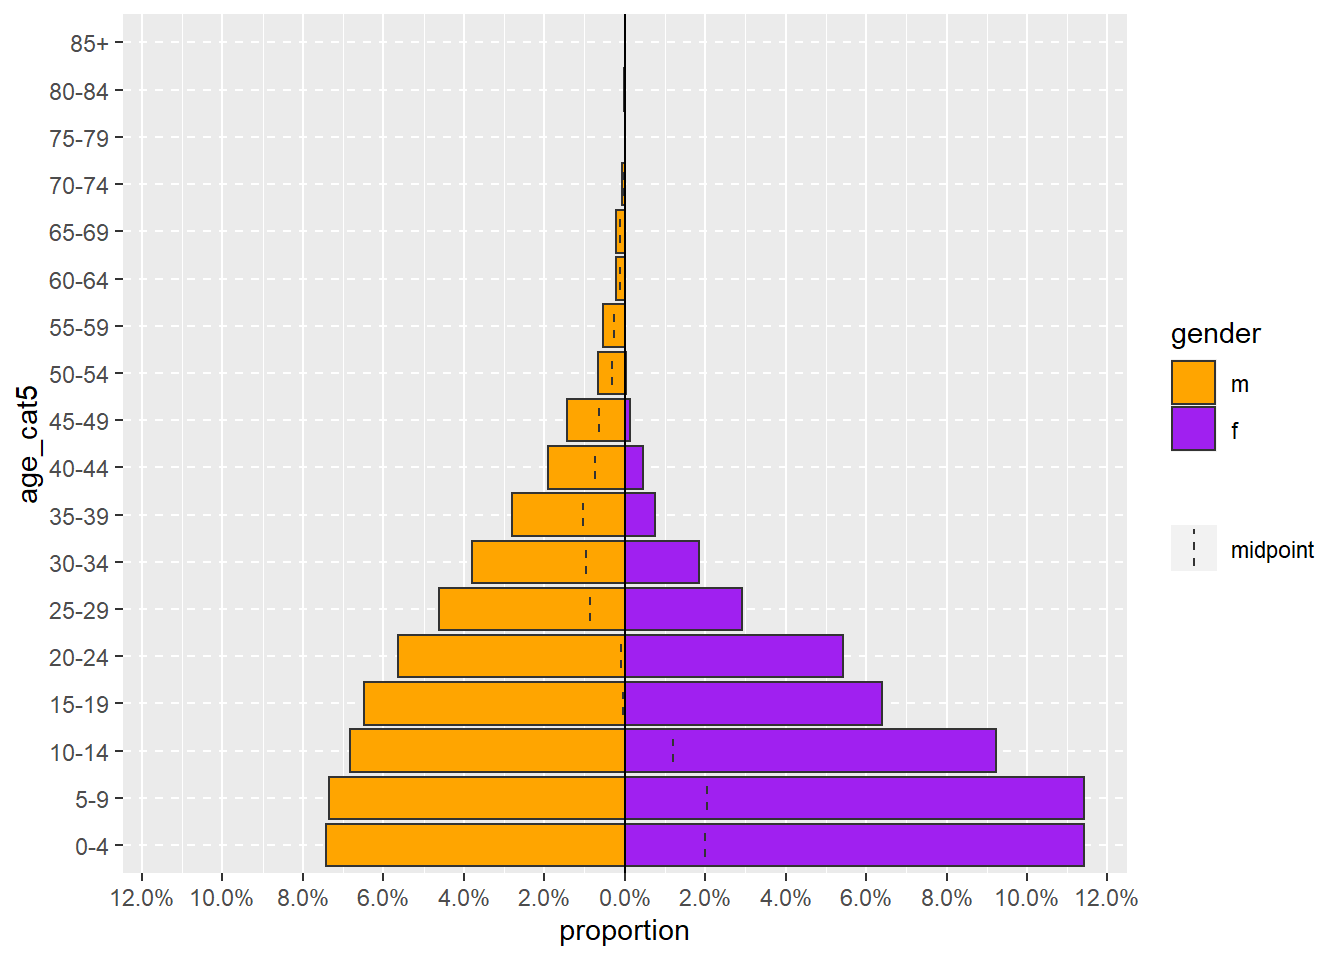
\includegraphics{C:/Users/Neale/ONEDRI~1/DOCUME~1/ANALYT~1/R/Projects/RHANDB~1/EPI_R_~1/pages_OUTPU~1/AGE_PY~1/figure-latex/unnamed-chunk-10-1.pdf}

\hypertarget{age_pyramid-with-aggregated-data}{%
\subsubsection{\texorpdfstring{\texttt{age\_pyramid()} with aggregated
data}{age\_pyramid() with aggregated data}}\label{age_pyramid-with-aggregated-data}}

The examples above assume your data are in a linelist-like format, with
one row per observation. If your data are already aggregated into counts
by age category, you can still use the \textbf{apyramid} package, as
shown below.

Let's say that your dataset looks like this, with columns for age
category, and male counts, female counts, and missing counts.\\
(see the handbook page on Transforming data for tips)

\begin{Shaded}
\begin{Highlighting}[]
\CommentTok{\# View the aggregated data}
\NormalTok{DT}\OperatorTok{::}\KeywordTok{datatable}\NormalTok{(demo\_agg, }\DataTypeTok{rownames =} \OtherTok{FALSE}\NormalTok{, }\DataTypeTok{filter=}\StringTok{"top"}\NormalTok{, }\DataTypeTok{options =} \KeywordTok{list}\NormalTok{(}\DataTypeTok{pageLength =} \DecValTok{5}\NormalTok{, }\DataTypeTok{scrollX=}\NormalTok{T) )}
\end{Highlighting}
\end{Shaded}

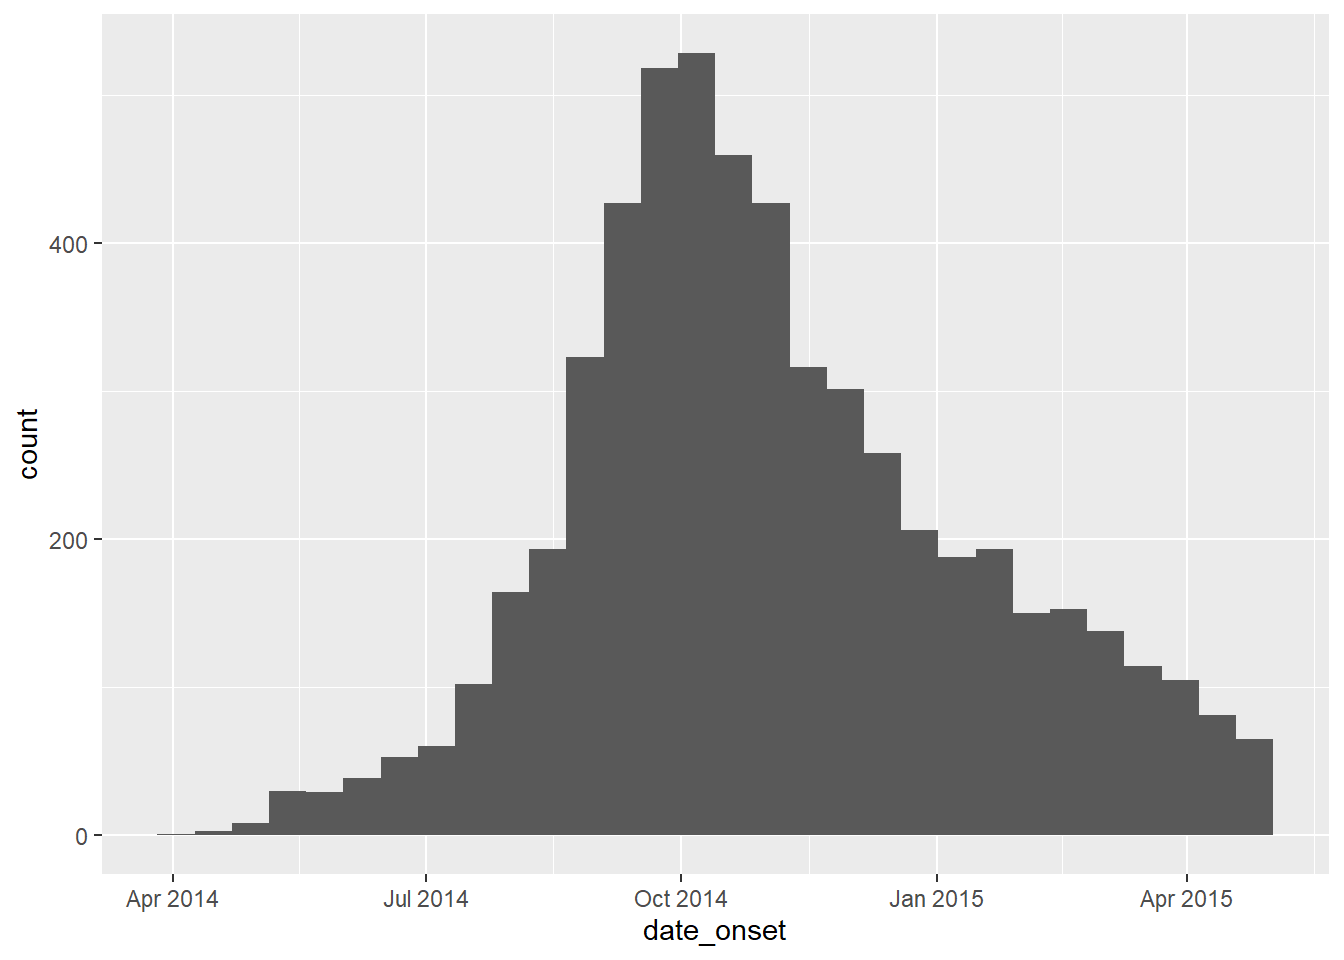
\includegraphics{C:/Users/Neale/ONEDRI~1/DOCUME~1/ANALYT~1/R/Projects/RHANDB~1/EPI_R_~1/pages_OUTPU~1/AGE_PY~1/figure-latex/unnamed-chunk-12-1.pdf}

\texttt{ggplot()} perfers data in ``long'' format, so first pivot the
data to be ``long'' with the \texttt{pivot\_longer()} function from
\textbf{dplyr}.

\begin{Shaded}
\begin{Highlighting}[]
\CommentTok{\# pivot the aggregated data into long format}
\NormalTok{demo\_agg\_long \textless{}{-}}\StringTok{ }\NormalTok{demo\_agg }\OperatorTok{\%\textgreater{}\%}\StringTok{ }
\StringTok{  }\KeywordTok{pivot\_longer}\NormalTok{(}\KeywordTok{c}\NormalTok{(f, m, missing\_gender),            }\CommentTok{\# cols to elongate}
               \DataTypeTok{names\_to =} \StringTok{"gender"}\NormalTok{,                }\CommentTok{\# name for new col of categories}
               \DataTypeTok{values\_to =} \StringTok{"counts"}\NormalTok{) }\OperatorTok{\%\textgreater{}\%}\StringTok{           }\CommentTok{\# name for new col of counts}
\StringTok{  }\KeywordTok{mutate}\NormalTok{(}\DataTypeTok{gender =} \KeywordTok{na\_if}\NormalTok{(gender, }\StringTok{"missing\_gender"}\NormalTok{)) }\CommentTok{\# convert "missing\_gender" to NA}
\end{Highlighting}
\end{Shaded}

\begin{Shaded}
\begin{Highlighting}[]
\CommentTok{\# View the aggregated data}
\NormalTok{DT}\OperatorTok{::}\KeywordTok{datatable}\NormalTok{(demo\_agg\_long, }\DataTypeTok{rownames =} \OtherTok{FALSE}\NormalTok{, }\DataTypeTok{filter=}\StringTok{"top"}\NormalTok{, }\DataTypeTok{options =} \KeywordTok{list}\NormalTok{(}\DataTypeTok{pageLength =} \DecValTok{5}\NormalTok{, }\DataTypeTok{scrollX=}\NormalTok{T) )}
\end{Highlighting}
\end{Shaded}

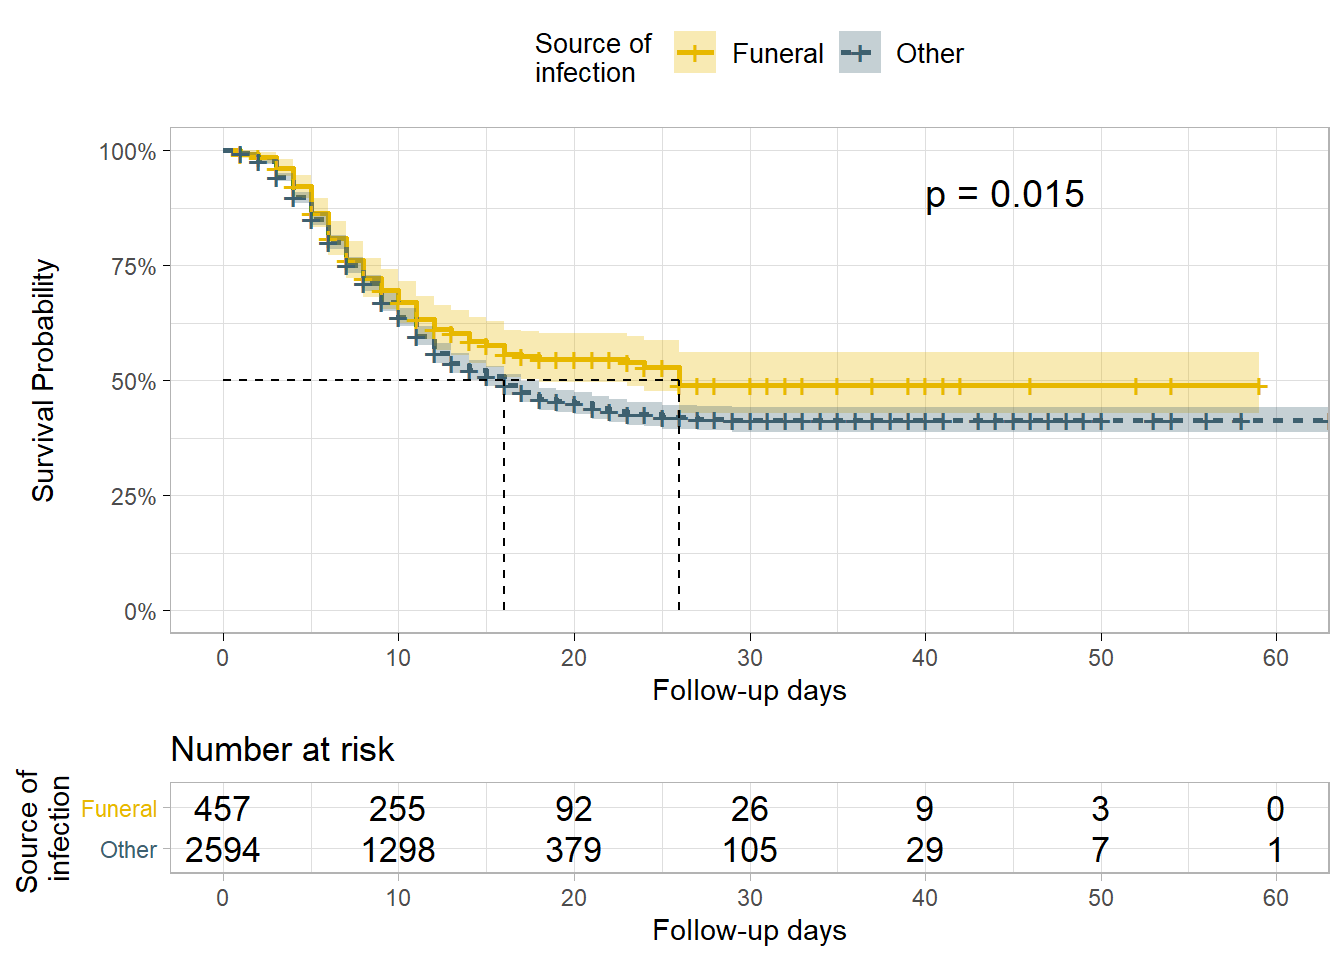
\includegraphics{C:/Users/Neale/ONEDRI~1/DOCUME~1/ANALYT~1/R/Projects/RHANDB~1/EPI_R_~1/pages_OUTPU~1/AGE_PY~1/figure-latex/unnamed-chunk-14-1.pdf}

Then use the \texttt{split\_by} and \texttt{count} arguments of
\texttt{age\_pyramid()} to specify the respective columns:

\begin{Shaded}
\begin{Highlighting}[]
\NormalTok{apyramid}\OperatorTok{::}\KeywordTok{age\_pyramid}\NormalTok{(}\DataTypeTok{data =}\NormalTok{ demo\_agg\_long,}
                      \DataTypeTok{age\_group =} \StringTok{"age\_cat5"}\NormalTok{,}
                      \DataTypeTok{split\_by =} \StringTok{"gender"}\NormalTok{,}
                      \DataTypeTok{count =} \StringTok{"counts"}\NormalTok{)      }\CommentTok{\# give the column name for the aggregated counts}
\end{Highlighting}
\end{Shaded}

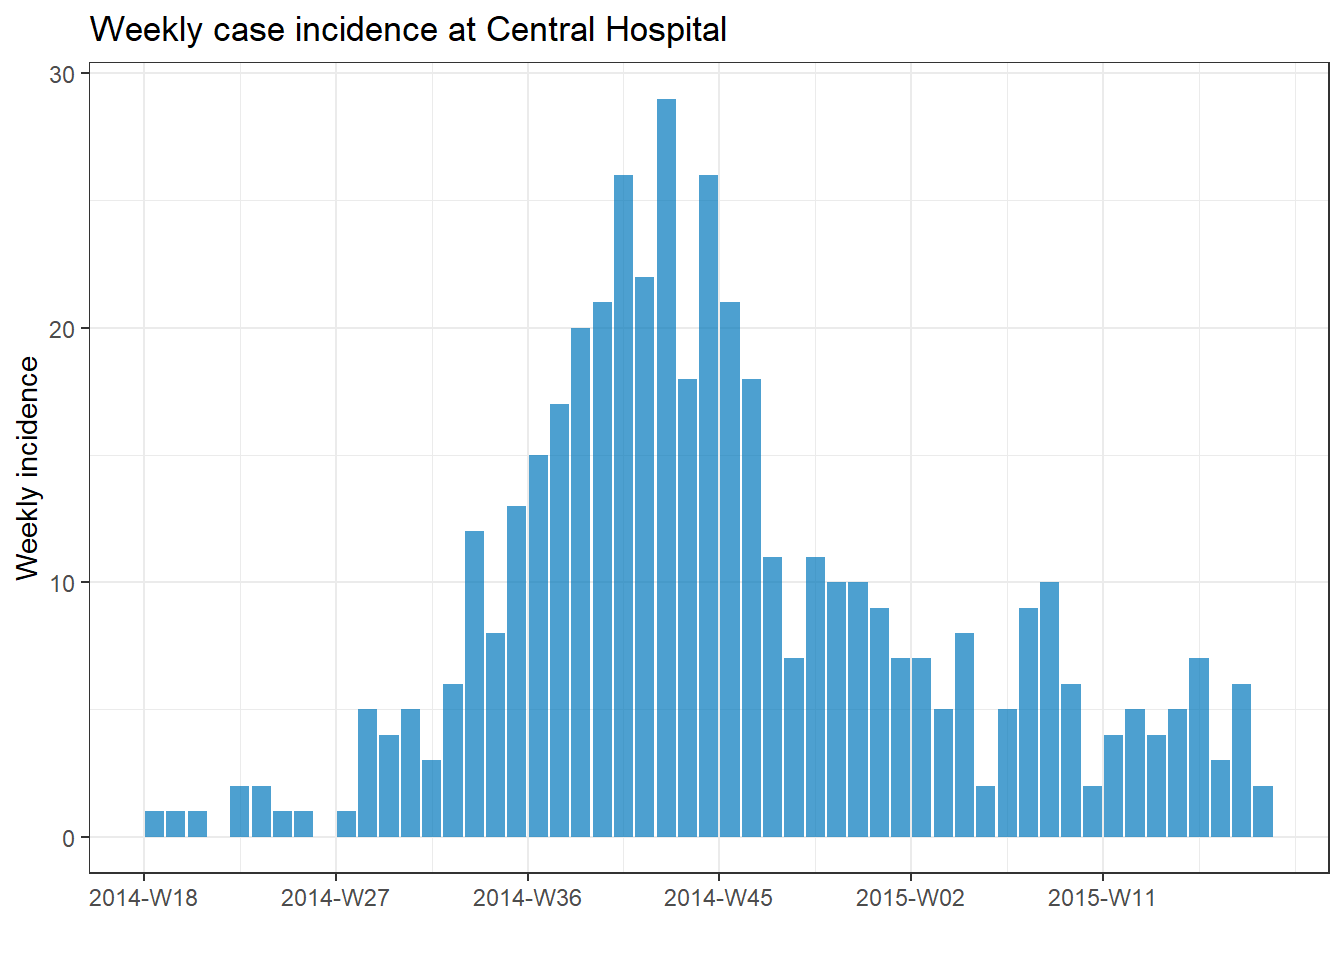
\includegraphics{C:/Users/Neale/ONEDRI~1/DOCUME~1/ANALYT~1/R/Projects/RHANDB~1/EPI_R_~1/pages_OUTPU~1/AGE_PY~1/figure-latex/unnamed-chunk-15-1.pdf}

Note in the above, that the factor order of ``m'' and ``f'' is different
(pyramid reversed). To adjust the order you must re-define gender in the
aggredated data as a Factor and order the levels as desired.

\hypertarget{ggplot}{%
\subsection{\texorpdfstring{\texttt{ggplot()}}{ggplot()}}\label{ggplot}}

Using \texttt{ggplot()} to build your age pyramid allows for more
flexibility, but requires more effort and understanding of how
\texttt{ggplot()} works. It is also easier to accidentally make
mistakes.

\textbf{apyramid} uses \texttt{ggplot()} in the background (and accepts
\texttt{ggplot()} commands added), but this page shows how to adjust or
recreate a pyramid only using \texttt{ggplot()}, if you wish.

\hypertarget{constructing-the-plot}{%
\subsubsection{Constructing the plot}\label{constructing-the-plot}}

First, understand that to make such a pyramid using \texttt{ggplot()}
the approach is to:

\begin{itemize}
\item
  Within the \texttt{ggplot()}, create \textbf{two} graphs by age
  category. Create one for each of the two grouping values (in this case
  gender). See filters applied to the \texttt{data} arguments in each
  \texttt{geom\_histogram()} commands below.
\item
  If using \texttt{geom\_histogram()}, the graphs operate off the
  numeric column (e.g.~\texttt{age\_years}), whereas if using
  \texttt{geom\_barplot()} the graphs operate from an ordered Factor
  (e.g.~\texttt{age\_cat5}).
\item
  One graph will have positive count values, while the other will have
  its counts converted to negative values - this allows both graphs to
  be seen and compared against each other in the same plot.
\item
  The command \texttt{coord\_flip()} switches the X and Y axes,
  resulting in the graphs turning vertical and creating the pyramid.
\item
  Lastly, the counts-axis labels must be specified so they appear as
  ``positive'' counts on both sides of the pyramid (despite the
  underlying values on one side being negative).
\end{itemize}

A \textbf{simple} version of this, using \texttt{geom\_histogram()}, is
below:

\begin{Shaded}
\begin{Highlighting}[]
  \CommentTok{\# begin ggplot}
  \KeywordTok{ggplot}\NormalTok{(}\DataTypeTok{data =}\NormalTok{ linelist, }\KeywordTok{aes}\NormalTok{(}\DataTypeTok{x =}\NormalTok{ age, }\DataTypeTok{fill =}\NormalTok{ gender)) }\OperatorTok{+}
\StringTok{  }
\StringTok{  }\CommentTok{\# female histogram}
\StringTok{  }\KeywordTok{geom\_histogram}\NormalTok{(}\DataTypeTok{data =} \KeywordTok{filter}\NormalTok{(linelist, gender }\OperatorTok{==}\StringTok{ "f"}\NormalTok{),}
                 \DataTypeTok{breaks =} \KeywordTok{seq}\NormalTok{(}\DecValTok{0}\NormalTok{,}\DecValTok{85}\NormalTok{,}\DecValTok{5}\NormalTok{),}
                 \DataTypeTok{colour =} \StringTok{"white"}\NormalTok{) }\OperatorTok{+}
\StringTok{  }
\StringTok{  }\CommentTok{\# male histogram (values converted to negative)}
\StringTok{  }\KeywordTok{geom\_histogram}\NormalTok{(}\DataTypeTok{data =} \KeywordTok{filter}\NormalTok{(linelist, gender }\OperatorTok{==}\StringTok{ "m"}\NormalTok{),}
                 \DataTypeTok{breaks =} \KeywordTok{seq}\NormalTok{(}\DecValTok{0}\NormalTok{,}\DecValTok{85}\NormalTok{,}\DecValTok{5}\NormalTok{),}
                 \KeywordTok{aes}\NormalTok{(}\DataTypeTok{y=}\NormalTok{..count..}\OperatorTok{*}\NormalTok{(}\OperatorTok{{-}}\DecValTok{1}\NormalTok{)),}
                 \DataTypeTok{colour =} \StringTok{"white"}\NormalTok{) }\OperatorTok{+}
\StringTok{  }
\StringTok{  }\CommentTok{\# flip the X and Y axes}
\StringTok{  }\KeywordTok{coord\_flip}\NormalTok{() }\OperatorTok{+}
\StringTok{  }
\StringTok{  }\CommentTok{\# adjust counts{-}axis scale}
\StringTok{  }\KeywordTok{scale\_y\_continuous}\NormalTok{(}\DataTypeTok{limits =} \KeywordTok{c}\NormalTok{(}\OperatorTok{{-}}\DecValTok{600}\NormalTok{, }\DecValTok{900}\NormalTok{),}
                     \DataTypeTok{breaks =} \KeywordTok{seq}\NormalTok{(}\OperatorTok{{-}}\DecValTok{600}\NormalTok{,}\DecValTok{900}\NormalTok{,}\DecValTok{100}\NormalTok{),}
                     \DataTypeTok{labels =} \KeywordTok{abs}\NormalTok{(}\KeywordTok{seq}\NormalTok{(}\OperatorTok{{-}}\DecValTok{600}\NormalTok{, }\DecValTok{900}\NormalTok{, }\DecValTok{100}\NormalTok{)))}
\end{Highlighting}
\end{Shaded}

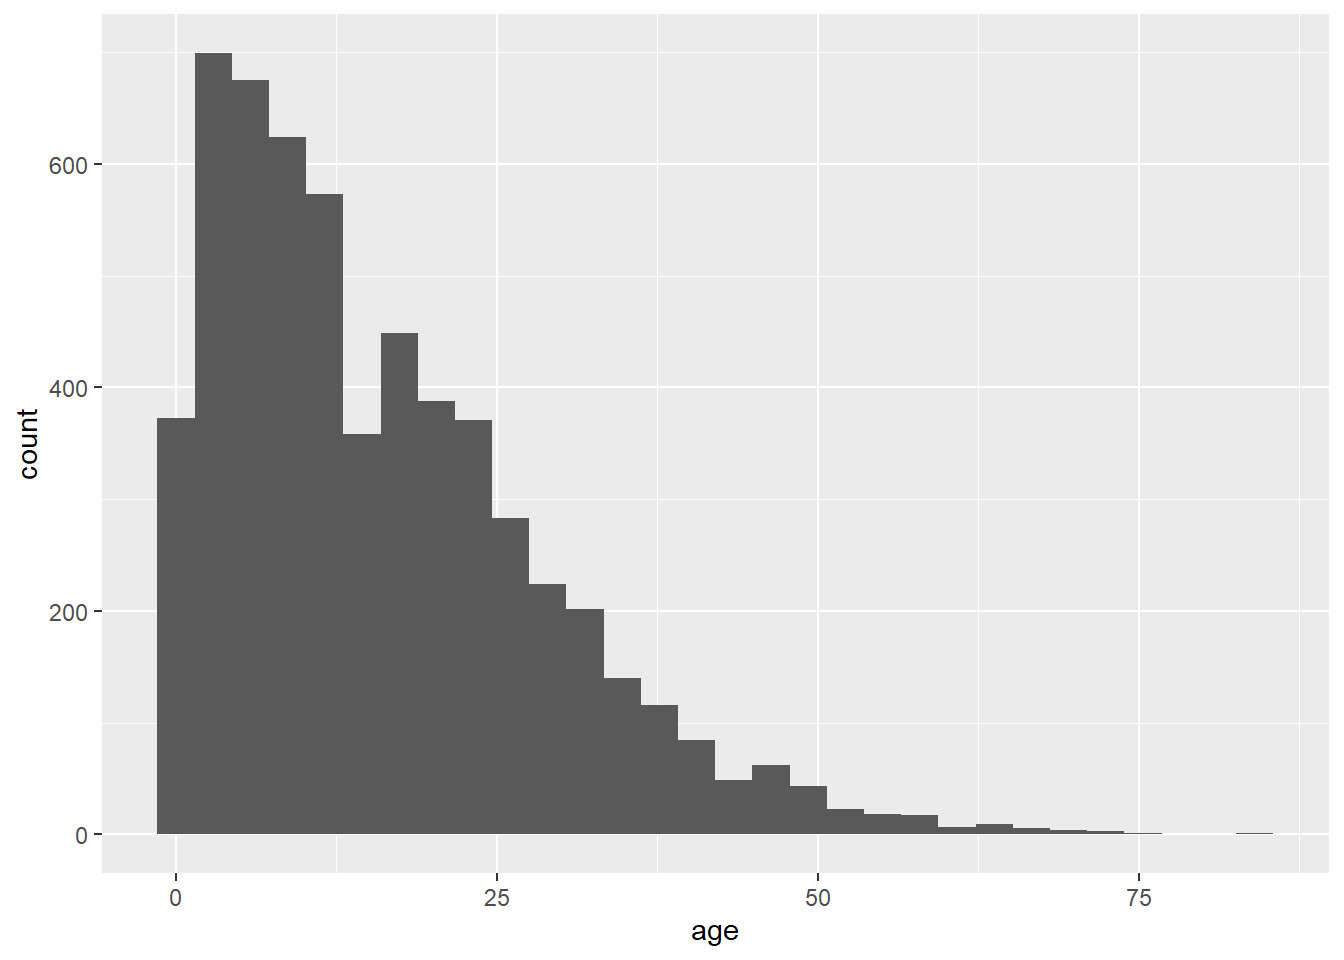
\includegraphics{C:/Users/Neale/ONEDRI~1/DOCUME~1/ANALYT~1/R/Projects/RHANDB~1/EPI_R_~1/pages_OUTPU~1/AGE_PY~1/figure-latex/unnamed-chunk-16-1.pdf}

{\textbf{\emph{DANGER:}} If the \textbf{limits} of your counts axis are
set too low, and a counts bar exceeds them, the bar will disappear
entirely or be artificially shortened! Watch for this if analyzing data
which is routinely updated. Prevent it by having your count-axis limits
auto-adjust to your data, as below.}

There are many things you can change/add to this simple version,
including:

\begin{itemize}
\tightlist
\item
  Auto adjust counts-axis count scale to your data (avoid errors
  discussed in warning below)\\
\item
  Manually specify colors and legend labels
\end{itemize}

\begin{Shaded}
\begin{Highlighting}[]
\CommentTok{\# create dataset with proportion of total}
\NormalTok{pyramid\_data \textless{}{-}}\StringTok{ }\NormalTok{linelist }\OperatorTok{\%\textgreater{}\%}
\StringTok{  }\KeywordTok{group\_by}\NormalTok{(age\_cat5, gender) }\OperatorTok{\%\textgreater{}\%}\StringTok{ }
\StringTok{  }\KeywordTok{summarize}\NormalTok{(}\DataTypeTok{counts =} \KeywordTok{n}\NormalTok{()) }\OperatorTok{\%\textgreater{}\%}\StringTok{ }
\StringTok{  }\KeywordTok{ungroup}\NormalTok{() }\OperatorTok{\%\textgreater{}\%}\StringTok{ }
\StringTok{  }\KeywordTok{mutate}\NormalTok{(}\DataTypeTok{percent =} \KeywordTok{round}\NormalTok{(}\DecValTok{100}\OperatorTok{*}\NormalTok{(counts }\OperatorTok{/}\StringTok{ }\KeywordTok{sum}\NormalTok{(counts, }\DataTypeTok{na.rm=}\NormalTok{T)),}\DecValTok{1}\NormalTok{), }
         \DataTypeTok{percent =} \KeywordTok{case\_when}\NormalTok{(}
\NormalTok{            gender }\OperatorTok{==}\StringTok{ "f"} \OperatorTok{\textasciitilde{}}\StringTok{ }\NormalTok{percent,}
\NormalTok{            gender }\OperatorTok{==}\StringTok{ "m"} \OperatorTok{\textasciitilde{}}\StringTok{ }\OperatorTok{{-}}\NormalTok{percent,}
            \OtherTok{TRUE}          \OperatorTok{\textasciitilde{}}\StringTok{ }\OtherTok{NA\_real\_}\NormalTok{))}

\NormalTok{max\_per \textless{}{-}}\StringTok{ }\KeywordTok{max}\NormalTok{(pyramid\_data}\OperatorTok{$}\NormalTok{percent, }\DataTypeTok{na.rm=}\NormalTok{T)}
\NormalTok{min\_per \textless{}{-}}\StringTok{ }\KeywordTok{min}\NormalTok{(pyramid\_data}\OperatorTok{$}\NormalTok{percent, }\DataTypeTok{na.rm=}\NormalTok{T)}


\CommentTok{\# begin ggplot}
  \KeywordTok{ggplot}\NormalTok{()}\OperatorTok{+}\StringTok{  }\CommentTok{\# default x{-}axis is age in years;}

\StringTok{  }\CommentTok{\# case data graph}
\StringTok{  }\KeywordTok{geom\_bar}\NormalTok{(}\DataTypeTok{data =}\NormalTok{ pyramid\_data,}
           \DataTypeTok{stat =} \StringTok{"identity"}\NormalTok{,}
           \KeywordTok{aes}\NormalTok{(}\DataTypeTok{x =}\NormalTok{ age\_cat5,}
               \DataTypeTok{y =}\NormalTok{ percent,}
               \DataTypeTok{fill =}\NormalTok{ gender),        }\CommentTok{\# }
           \DataTypeTok{colour =} \StringTok{"white"}\NormalTok{)}\OperatorTok{+}\StringTok{         }\CommentTok{\# white around each bar}
\StringTok{  }
\StringTok{  }\CommentTok{\# flip the X and Y axes to make pyramid vertical}
\StringTok{  }\KeywordTok{coord\_flip}\NormalTok{()}\OperatorTok{+}
\StringTok{  }

\StringTok{  }\CommentTok{\# adjust the axes scales (remember they are flipped now!)}
\StringTok{  }\CommentTok{\#scale\_x\_continuous(breaks = seq(0,100,5), labels = seq(0,100,5)) +}
\StringTok{  }\KeywordTok{scale\_y\_continuous}\NormalTok{(}\DataTypeTok{limits =} \KeywordTok{c}\NormalTok{(min\_per, max\_per),}
                     \DataTypeTok{breaks =} \KeywordTok{seq}\NormalTok{(}\KeywordTok{floor}\NormalTok{(min\_per), }\KeywordTok{ceiling}\NormalTok{(max\_per), }\DecValTok{2}\NormalTok{),}
                     \DataTypeTok{labels =} \KeywordTok{paste0}\NormalTok{(}\KeywordTok{abs}\NormalTok{(}\KeywordTok{seq}\NormalTok{(}\KeywordTok{floor}\NormalTok{(min\_per), }\KeywordTok{ceiling}\NormalTok{(max\_per), }\DecValTok{2}\NormalTok{)), }\StringTok{"\%"}\NormalTok{))}\OperatorTok{+}

\StringTok{  }\CommentTok{\# designate colors and legend labels manually}
\StringTok{  }\KeywordTok{scale\_fill\_manual}\NormalTok{(}
    \DataTypeTok{values =} \KeywordTok{c}\NormalTok{(}\StringTok{"f"}\NormalTok{ =}\StringTok{ "orange"}\NormalTok{,}
               \StringTok{"m"}\NormalTok{ =}\StringTok{ "darkgreen"}\NormalTok{),}
    \DataTypeTok{labels =} \KeywordTok{c}\NormalTok{(}\StringTok{"Female"}\NormalTok{, }\StringTok{"Male"}\NormalTok{),}
\NormalTok{  ) }\OperatorTok{+}
\StringTok{  }
\StringTok{  }\CommentTok{\# label values (remember X and Y flipped now)}
\StringTok{  }\KeywordTok{labs}\NormalTok{(}
    \DataTypeTok{x =} \StringTok{"Age group"}\NormalTok{,}
    \DataTypeTok{y =} \StringTok{"Percent of total"}\NormalTok{,}
    \DataTypeTok{fill =} \OtherTok{NULL}\NormalTok{,}
    \DataTypeTok{caption =}\NormalTok{ stringr}\OperatorTok{::}\KeywordTok{str\_glue}\NormalTok{(}\StringTok{"Data are from linelist }\CharTok{\textbackslash{}n}\StringTok{n = \{nrow(linelist)\} (age or sex missing for \{sum(is.na(linelist$gender) | is.na(linelist$age\_years))\} cases) }\CharTok{\textbackslash{}n}\StringTok{Data as of: \{format(Sys.Date(), \textquotesingle{}\%d \%b \%Y\textquotesingle{})\}"}\NormalTok{)) }\OperatorTok{+}
\StringTok{  }
\StringTok{  }\CommentTok{\# optional aesthetic themes}
\StringTok{  }\KeywordTok{theme}\NormalTok{(}
    \DataTypeTok{panel.grid.major =} \KeywordTok{element\_blank}\NormalTok{(),}
    \DataTypeTok{panel.grid.minor =} \KeywordTok{element\_blank}\NormalTok{(),}
    \DataTypeTok{panel.background =} \KeywordTok{element\_blank}\NormalTok{(),}
    \DataTypeTok{axis.line =} \KeywordTok{element\_line}\NormalTok{(}\DataTypeTok{colour =} \StringTok{"black"}\NormalTok{),}
    \DataTypeTok{plot.title =} \KeywordTok{element\_text}\NormalTok{(}\DataTypeTok{hjust =} \FloatTok{0.5}\NormalTok{), }
    \DataTypeTok{plot.caption =} \KeywordTok{element\_text}\NormalTok{(}\DataTypeTok{hjust=}\DecValTok{0}\NormalTok{, }\DataTypeTok{size=}\DecValTok{11}\NormalTok{, }\DataTypeTok{face =} \StringTok{"italic"}\NormalTok{)) }\OperatorTok{+}\StringTok{ }
\StringTok{  }
\StringTok{  }\KeywordTok{ggtitle}\NormalTok{(}\KeywordTok{paste0}\NormalTok{(}\StringTok{"Age and gender of cases"}\NormalTok{))}
\end{Highlighting}
\end{Shaded}

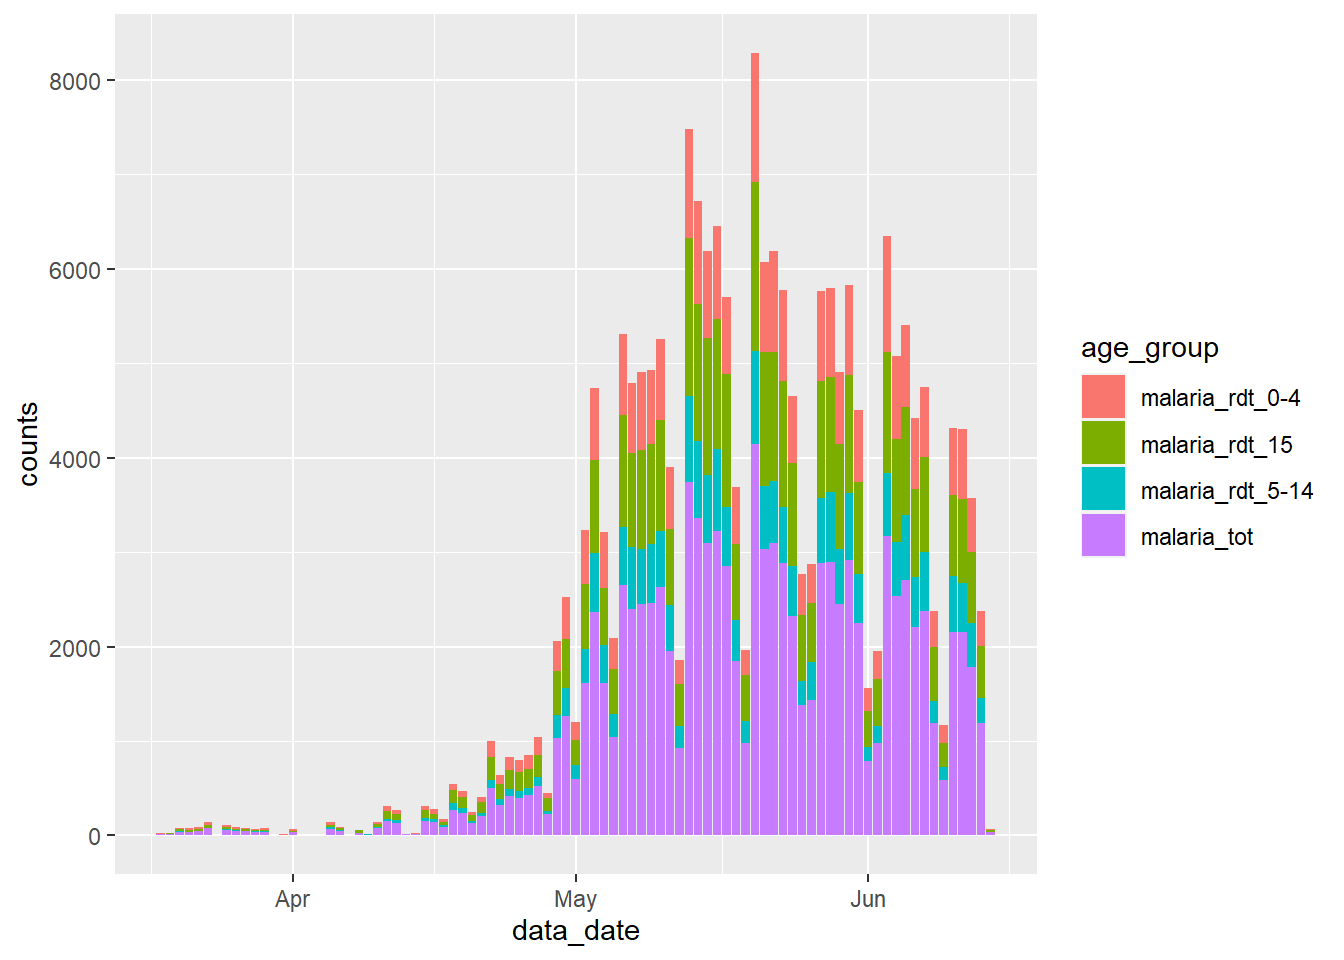
\includegraphics{C:/Users/Neale/ONEDRI~1/DOCUME~1/ANALYT~1/R/Projects/RHANDB~1/EPI_R_~1/pages_OUTPU~1/AGE_PY~1/figure-latex/unnamed-chunk-17-1.pdf}

\hypertarget{compare-to-expected-demographics}{%
\subsubsection{Compare to expected
demographics}\label{compare-to-expected-demographics}}

With the flexibility of \texttt{ggplot()}, you can have a second layer
of bars in the background that represent the true population pyramid.
This can provide a nice visualization to compare the observed counts
with the baseline.

Import and view the population data

\begin{Shaded}
\begin{Highlighting}[]
\CommentTok{\# import the population demographics data}
\NormalTok{pop \textless{}{-}}\StringTok{ }\NormalTok{rio}\OperatorTok{::}\KeywordTok{import}\NormalTok{(}\StringTok{"country\_demographics.csv"}\NormalTok{)}
\end{Highlighting}
\end{Shaded}

\begin{Shaded}
\begin{Highlighting}[]
\CommentTok{\# display the linelist data as a table}
\NormalTok{DT}\OperatorTok{::}\KeywordTok{datatable}\NormalTok{(pop, }\DataTypeTok{rownames =} \OtherTok{FALSE}\NormalTok{, }\DataTypeTok{filter=}\StringTok{"top"}\NormalTok{, }\DataTypeTok{options =} \KeywordTok{list}\NormalTok{(}\DataTypeTok{pageLength =} \DecValTok{10}\NormalTok{, }\DataTypeTok{scrollX=}\NormalTok{T) )}
\end{Highlighting}
\end{Shaded}

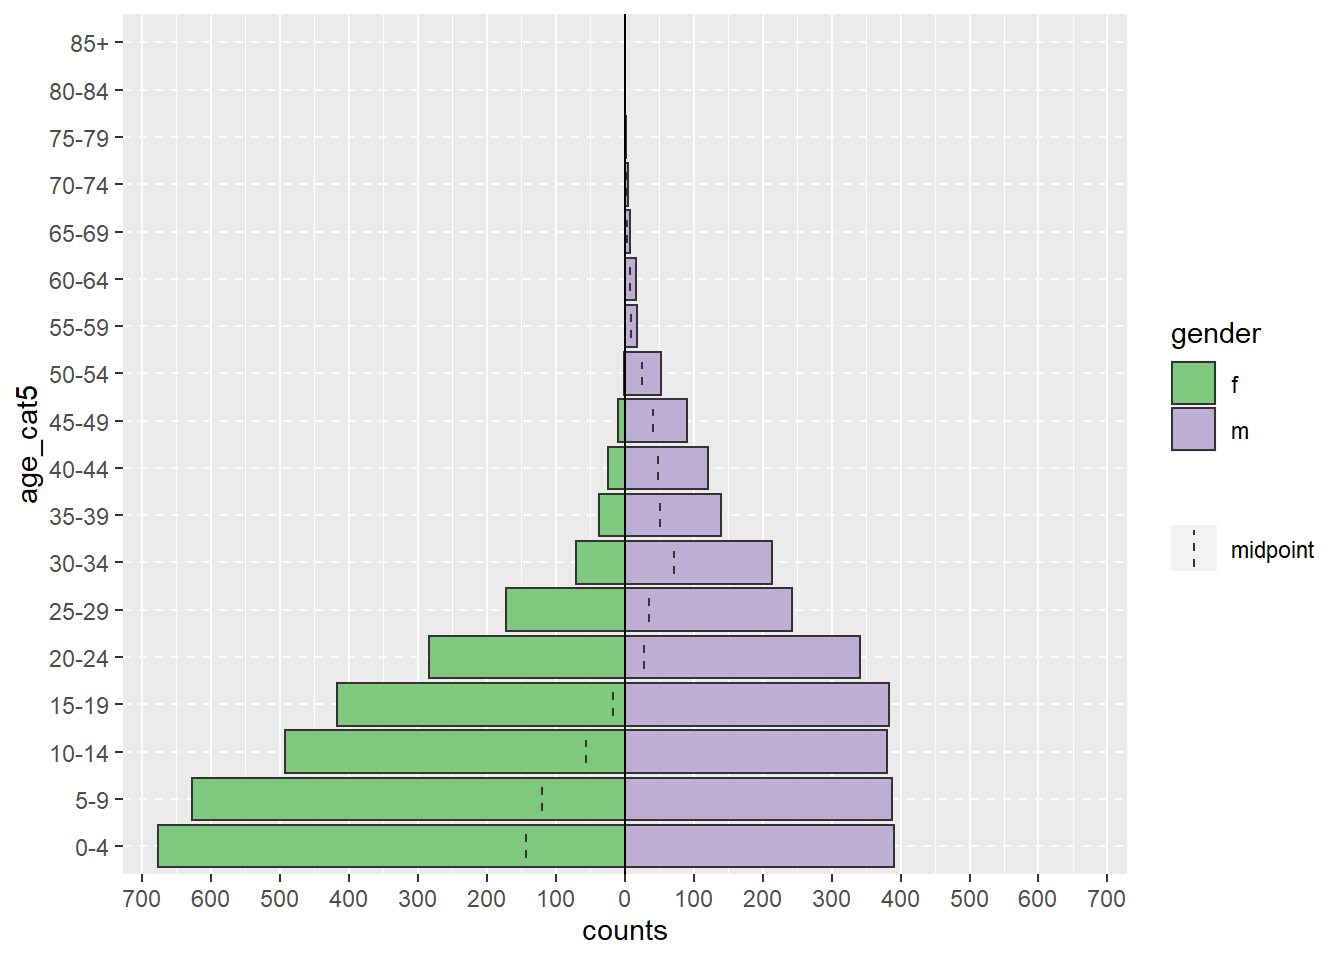
\includegraphics{C:/Users/Neale/ONEDRI~1/DOCUME~1/ANALYT~1/R/Projects/RHANDB~1/EPI_R_~1/pages_OUTPU~1/AGE_PY~1/figure-latex/unnamed-chunk-20-1.pdf}
First some data management steps:

Here we record the order of age categories that we want to appear. Due
to some quirks the way the \texttt{ggplot()} is implemented, it is
easiest to store these as a character vector and use them later in the
plotting function.

\begin{Shaded}
\begin{Highlighting}[]
\CommentTok{\# record correct age cat levels}
\NormalTok{age\_levels \textless{}{-}}\StringTok{ }\KeywordTok{c}\NormalTok{(}\StringTok{"0{-}4"}\NormalTok{,}\StringTok{"5{-}9"}\NormalTok{, }\StringTok{"10{-}14"}\NormalTok{, }\StringTok{"15{-}19"}\NormalTok{, }\StringTok{"20{-}24"}\NormalTok{,}
                \StringTok{"25{-}29"}\NormalTok{,}\StringTok{"30{-}34"}\NormalTok{, }\StringTok{"35{-}39"}\NormalTok{, }\StringTok{"40{-}44"}\NormalTok{, }\StringTok{"45{-}49"}\NormalTok{,}
                \StringTok{"50{-}54"}\NormalTok{, }\StringTok{"55{-}59"}\NormalTok{, }\StringTok{"60{-}64"}\NormalTok{, }\StringTok{"65{-}69"}\NormalTok{, }\StringTok{"70{-}74"}\NormalTok{,}
                \StringTok{"75{-}79"}\NormalTok{, }\StringTok{"80{-}84"}\NormalTok{, }\StringTok{"85+"}\NormalTok{)}
\end{Highlighting}
\end{Shaded}

Combine the population and case data through the \textbf{dplyr} function
\texttt{bind\_rows()}:

\begin{itemize}
\tightlist
\item
  First, ensure they have the \emph{exact same} column names, age
  categories values, and gender values\\
\item
  Make them have the same data structure: columns of age category,
  gender, counts, and percent of total\\
\item
  Bind them together, one on-top of the other (\texttt{bind\_rows()})
\end{itemize}

\begin{Shaded}
\begin{Highlighting}[]
\CommentTok{\# create/transform populaton data, with percent of total}
\CommentTok{\#\#\#\#\#\#\#\#\#\#\#\#\#\#\#\#\#\#\#\#\#\#\#\#\#\#\#\#\#\#\#\#\#\#\#\#\#\#\#\#\#\#\#\#\#\#\#\#\#\#\#\#\#\#\#\#}
\NormalTok{pop\_data \textless{}{-}}\StringTok{ }\KeywordTok{pivot\_longer}\NormalTok{(pop, }\KeywordTok{c}\NormalTok{(m, f), }\DataTypeTok{names\_to =} \StringTok{"gender"}\NormalTok{, }\DataTypeTok{values\_to =} \StringTok{"counts"}\NormalTok{) }\OperatorTok{\%\textgreater{}\%}\StringTok{ }\CommentTok{\# pivot gender columns longer}
\StringTok{  }\KeywordTok{mutate}\NormalTok{(}\DataTypeTok{data =} \StringTok{"population"}\NormalTok{,                                                         }\CommentTok{\# add column designating data source}
         \DataTypeTok{percent  =} \KeywordTok{round}\NormalTok{(}\DecValTok{100}\OperatorTok{*}\NormalTok{(counts }\OperatorTok{/}\StringTok{ }\KeywordTok{sum}\NormalTok{(counts, }\DataTypeTok{na.rm=}\NormalTok{T)),}\DecValTok{1}\NormalTok{),                     }\CommentTok{\# calculate \% of total}
         \DataTypeTok{percent  =} \KeywordTok{case\_when}\NormalTok{(                                                        }\CommentTok{\# if male, convert \% to negative}
\NormalTok{                            gender }\OperatorTok{==}\StringTok{ "f"} \OperatorTok{\textasciitilde{}}\StringTok{ }\NormalTok{percent,}
\NormalTok{                            gender }\OperatorTok{==}\StringTok{ "m"} \OperatorTok{\textasciitilde{}}\StringTok{ }\OperatorTok{{-}}\NormalTok{percent,}
                            \OtherTok{TRUE}          \OperatorTok{\textasciitilde{}}\StringTok{ }\OtherTok{NA\_real\_}\NormalTok{))}
\end{Highlighting}
\end{Shaded}

Review the changed population dataset

\begin{Shaded}
\begin{Highlighting}[]
\CommentTok{\# display the linelist data as a table}
\NormalTok{DT}\OperatorTok{::}\KeywordTok{datatable}\NormalTok{(pop\_data, }\DataTypeTok{rownames =} \OtherTok{FALSE}\NormalTok{, }\DataTypeTok{filter=}\StringTok{"top"}\NormalTok{, }\DataTypeTok{options =} \KeywordTok{list}\NormalTok{(}\DataTypeTok{pageLength =} \DecValTok{5}\NormalTok{, }\DataTypeTok{scrollX=}\NormalTok{T) )}
\end{Highlighting}
\end{Shaded}

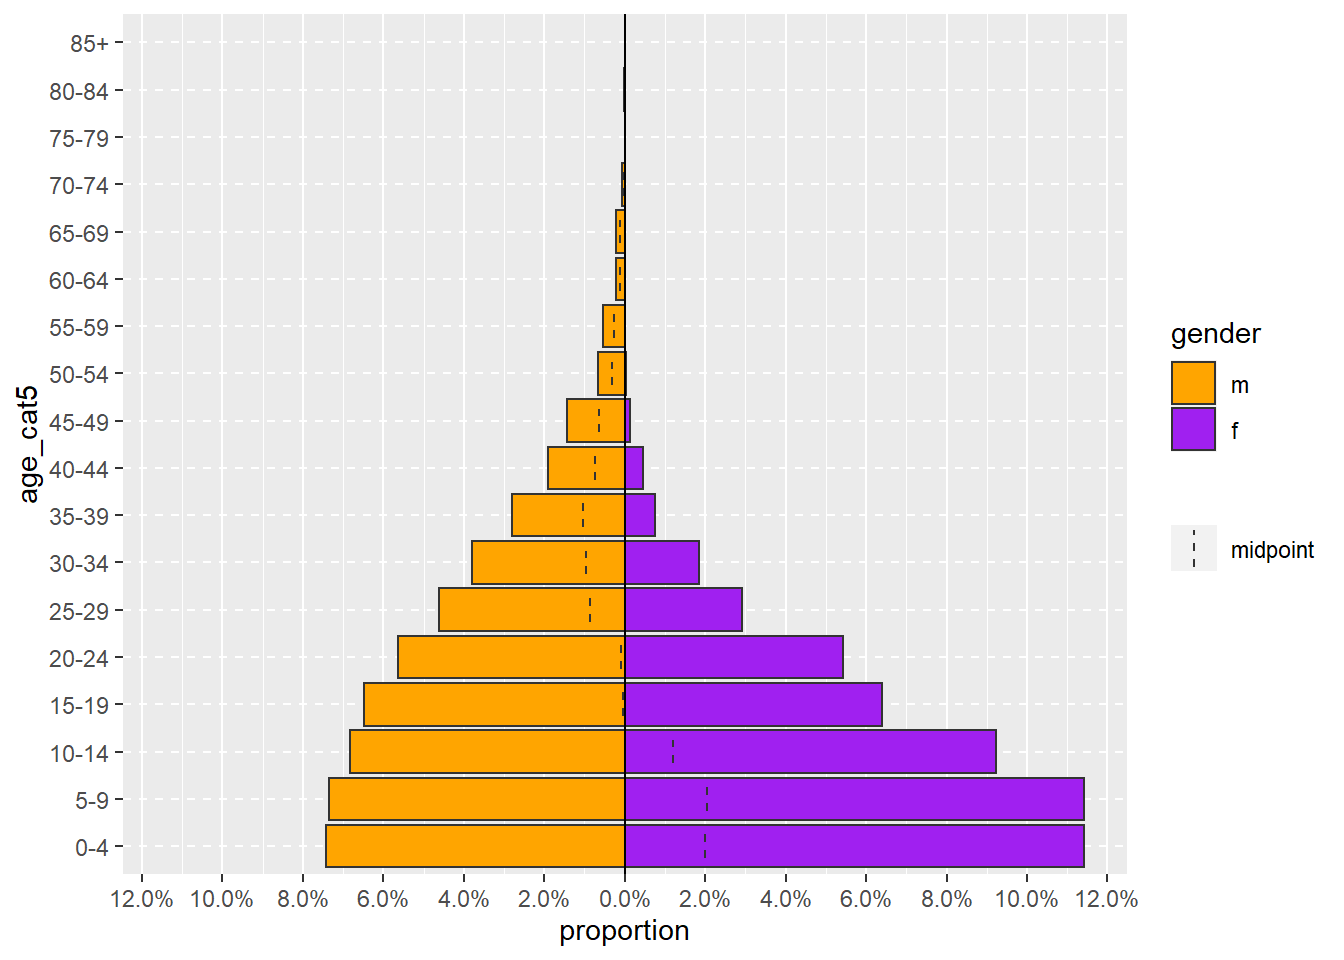
\includegraphics{C:/Users/Neale/ONEDRI~1/DOCUME~1/ANALYT~1/R/Projects/RHANDB~1/EPI_R_~1/pages_OUTPU~1/AGE_PY~1/figure-latex/unnamed-chunk-23-1.pdf}

Now implement the same for the case linelist. Slightly different because
it begins with case-rows, not counts.

\begin{Shaded}
\begin{Highlighting}[]
\CommentTok{\# create case data by age/gender, with percent of total}
\CommentTok{\#\#\#\#\#\#\#\#\#\#\#\#\#\#\#\#\#\#\#\#\#\#\#\#\#\#\#\#\#\#\#\#\#\#\#\#\#\#\#\#\#\#\#\#\#\#\#\#\#\#\#\#\#\#\#}
\NormalTok{case\_data \textless{}{-}}\StringTok{ }\NormalTok{linelist }\OperatorTok{\%\textgreater{}\%}
\StringTok{  }\KeywordTok{group\_by}\NormalTok{(age\_cat5, gender) }\OperatorTok{\%\textgreater{}\%}\StringTok{  }\CommentTok{\# aggregate linelist cases into age{-}gender groups}
\StringTok{  }\KeywordTok{summarize}\NormalTok{(}\DataTypeTok{counts =} \KeywordTok{n}\NormalTok{()) }\OperatorTok{\%\textgreater{}\%}\StringTok{     }\CommentTok{\# calculate counts per age{-}gender group}
\StringTok{  }\KeywordTok{ungroup}\NormalTok{() }\OperatorTok{\%\textgreater{}\%}\StringTok{ }
\StringTok{  }\KeywordTok{mutate}\NormalTok{(}\DataTypeTok{data =} \StringTok{"cases"}\NormalTok{,                                          }\CommentTok{\# add column designating data source}
         \DataTypeTok{percent =} \KeywordTok{round}\NormalTok{(}\DecValTok{100}\OperatorTok{*}\NormalTok{(counts }\OperatorTok{/}\StringTok{ }\KeywordTok{sum}\NormalTok{(counts, }\DataTypeTok{na.rm=}\NormalTok{T)),}\DecValTok{1}\NormalTok{),  }\CommentTok{\# calculate \% of total for age{-}gender groups}
         \DataTypeTok{percent =} \KeywordTok{case\_when}\NormalTok{(                                     }\CommentTok{\# convert \% to negative if male}
\NormalTok{            gender }\OperatorTok{==}\StringTok{ "f"} \OperatorTok{\textasciitilde{}}\StringTok{ }\NormalTok{percent,}
\NormalTok{            gender }\OperatorTok{==}\StringTok{ "m"} \OperatorTok{\textasciitilde{}}\StringTok{ }\OperatorTok{{-}}\NormalTok{percent,}
            \OtherTok{TRUE}          \OperatorTok{\textasciitilde{}}\StringTok{ }\OtherTok{NA\_real\_}\NormalTok{))}
\end{Highlighting}
\end{Shaded}

Review the changed case dataset

\begin{Shaded}
\begin{Highlighting}[]
\CommentTok{\# display the linelist data as a table}
\NormalTok{DT}\OperatorTok{::}\KeywordTok{datatable}\NormalTok{(case\_data, }\DataTypeTok{rownames =} \OtherTok{FALSE}\NormalTok{, }\DataTypeTok{filter=}\StringTok{"top"}\NormalTok{, }\DataTypeTok{options =} \KeywordTok{list}\NormalTok{(}\DataTypeTok{pageLength =} \DecValTok{5}\NormalTok{, }\DataTypeTok{scrollX=}\NormalTok{T) )}
\end{Highlighting}
\end{Shaded}

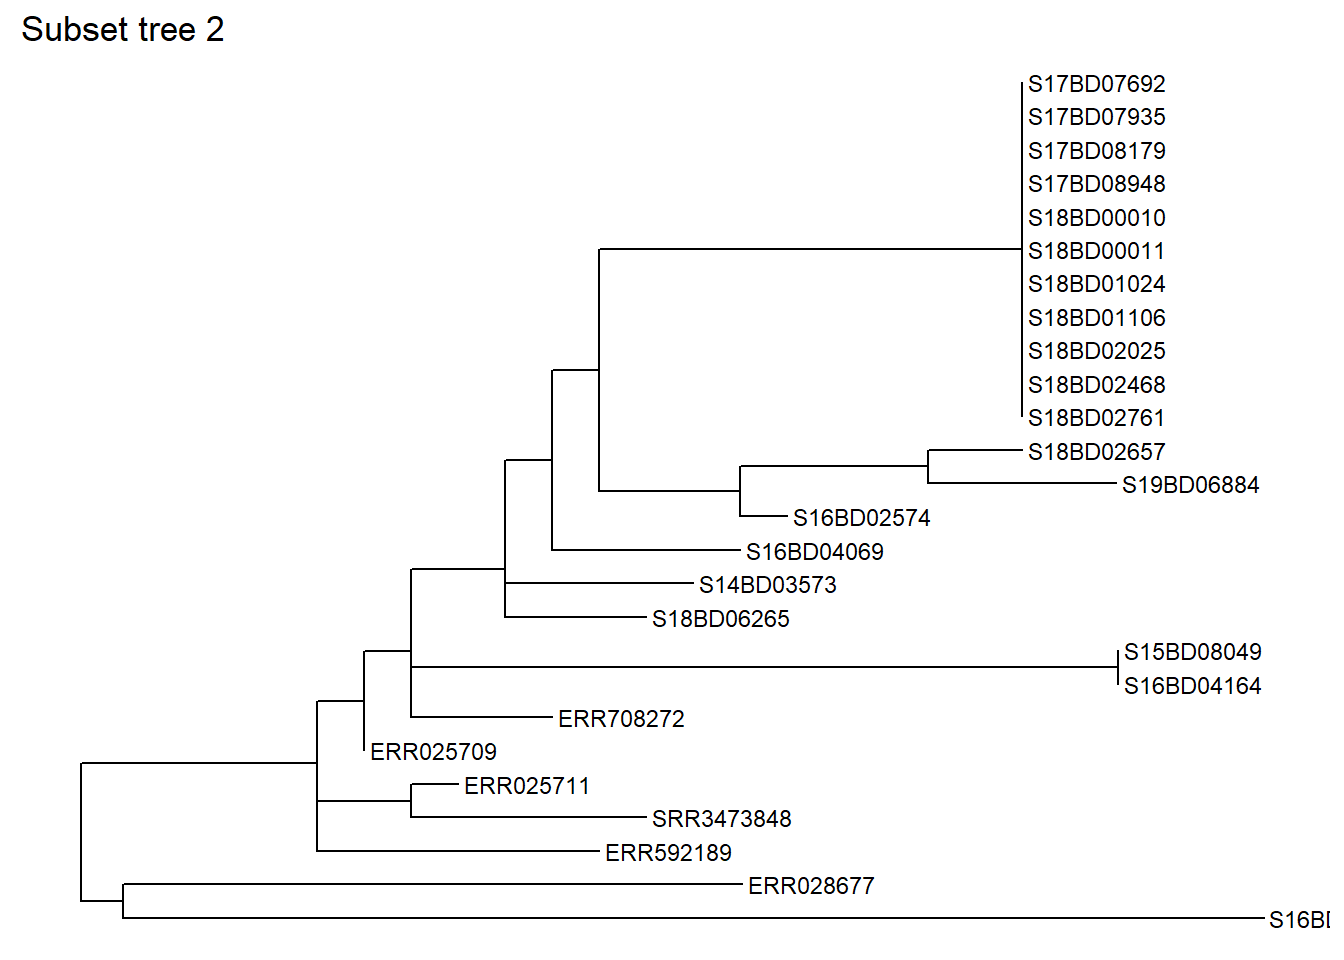
\includegraphics{C:/Users/Neale/ONEDRI~1/DOCUME~1/ANALYT~1/R/Projects/RHANDB~1/EPI_R_~1/pages_OUTPU~1/AGE_PY~1/figure-latex/unnamed-chunk-25-1.pdf}
Now the two datasets are combined, one on top of the other (same column
names)

\begin{Shaded}
\begin{Highlighting}[]
\CommentTok{\# combine case and population data (same column names, age\_cat values, and gender values)}
\NormalTok{pyramid\_data \textless{}{-}}\StringTok{ }\KeywordTok{bind\_rows}\NormalTok{(case\_data, pop\_data)}
\end{Highlighting}
\end{Shaded}

Store the maximum and minimum percent values, used in the plotting
funtion to define the extent of the plot (and not cut off any bars!)

\begin{Shaded}
\begin{Highlighting}[]
\CommentTok{\# Define extent of percent axis, used for plot limits}
\NormalTok{max\_per \textless{}{-}}\StringTok{ }\KeywordTok{max}\NormalTok{(pyramid\_data}\OperatorTok{$}\NormalTok{percent, }\DataTypeTok{na.rm=}\NormalTok{T)}
\NormalTok{min\_per \textless{}{-}}\StringTok{ }\KeywordTok{min}\NormalTok{(pyramid\_data}\OperatorTok{$}\NormalTok{percent, }\DataTypeTok{na.rm=}\NormalTok{T)}
\end{Highlighting}
\end{Shaded}

Now the plot is made with \texttt{ggplot()}:

\begin{itemize}
\tightlist
\item
  One bar graph of population data (wider, more transparent bars)
\item
  One bar graph of case data (small, more solid bars)
\end{itemize}

\begin{Shaded}
\begin{Highlighting}[]

\CommentTok{\# begin ggplot}
\CommentTok{\#\#\#\#\#\#\#\#\#\#\#\#\#\#}
\KeywordTok{ggplot}\NormalTok{()}\OperatorTok{+}\StringTok{  }\CommentTok{\# default x{-}axis is age in years;}

\StringTok{  }\CommentTok{\# population data graph}
\StringTok{  }\KeywordTok{geom\_bar}\NormalTok{(}\DataTypeTok{data =} \KeywordTok{filter}\NormalTok{(pyramid\_data, data }\OperatorTok{==}\StringTok{ "population"}\NormalTok{),}
           \DataTypeTok{stat =} \StringTok{"identity"}\NormalTok{,}
           \KeywordTok{aes}\NormalTok{(}\DataTypeTok{x =}\NormalTok{ age\_cat5,}
               \DataTypeTok{y =}\NormalTok{ percent,}
               \DataTypeTok{fill =}\NormalTok{ gender),        }
           \DataTypeTok{colour =} \StringTok{"black"}\NormalTok{,                               }\CommentTok{\# black color around bars}
           \DataTypeTok{alpha =} \FloatTok{0.2}\NormalTok{,                                    }\CommentTok{\# more transparent}
           \DataTypeTok{width =} \DecValTok{1}\NormalTok{)}\OperatorTok{+}\StringTok{                                     }\CommentTok{\# full width}
\StringTok{  }
\StringTok{  }\CommentTok{\# case data graph}
\StringTok{  }\KeywordTok{geom\_bar}\NormalTok{(}\DataTypeTok{data =} \KeywordTok{filter}\NormalTok{(pyramid\_data, data }\OperatorTok{==}\StringTok{ "cases"}\NormalTok{), }
           \DataTypeTok{stat =} \StringTok{"identity"}\NormalTok{,                              }\CommentTok{\# use \% as given in data, not counting rows}
           \KeywordTok{aes}\NormalTok{(}\DataTypeTok{x =}\NormalTok{ age\_cat5,                               }\CommentTok{\# age categories as original X axis}
               \DataTypeTok{y =}\NormalTok{ percent,                                }\CommentTok{\# \% as original Y{-}axis}
               \DataTypeTok{fill =}\NormalTok{ gender),                             }\CommentTok{\# fill of bars by gender}
           \DataTypeTok{colour =} \StringTok{"black"}\NormalTok{,                               }\CommentTok{\# black color around bars}
           \DataTypeTok{alpha =} \DecValTok{1}\NormalTok{,                                      }\CommentTok{\# not transparent }
           \DataTypeTok{width =} \FloatTok{0.3}\NormalTok{)}\OperatorTok{+}\StringTok{                                   }\CommentTok{\# half width}
\StringTok{  }
\StringTok{  }\CommentTok{\# flip the X and Y axes to make pyramid vertical}
\StringTok{  }\KeywordTok{coord\_flip}\NormalTok{()}\OperatorTok{+}
\StringTok{  }
\StringTok{  }\CommentTok{\# adjust axes order, scale, and labels (remember X and Y axes are flipped now)}
\StringTok{  }\CommentTok{\# manually ensure that age{-}axis is ordered correctly}
\StringTok{  }\KeywordTok{scale\_x\_discrete}\NormalTok{(}\DataTypeTok{limits =}\NormalTok{ age\_levels)}\OperatorTok{+}\StringTok{ }
\StringTok{  }
\StringTok{  }\CommentTok{\# set percent{-}axis }
\StringTok{  }\KeywordTok{scale\_y\_continuous}\NormalTok{(}\DataTypeTok{limits =} \KeywordTok{c}\NormalTok{(min\_per, max\_per),                                          }\CommentTok{\# min and max defined above}
                     \DataTypeTok{breaks =} \KeywordTok{seq}\NormalTok{(}\KeywordTok{floor}\NormalTok{(min\_per), }\KeywordTok{ceiling}\NormalTok{(max\_per), }\DataTypeTok{by =} \DecValTok{2}\NormalTok{),                }\CommentTok{\# from min\% to max\% by 2 }
                     \DataTypeTok{labels =} \KeywordTok{paste0}\NormalTok{(                                                       }\CommentTok{\# for the labels, paste together... }
                       \KeywordTok{abs}\NormalTok{(}\KeywordTok{seq}\NormalTok{(}\KeywordTok{floor}\NormalTok{(min\_per), }\KeywordTok{ceiling}\NormalTok{(max\_per), }\DataTypeTok{by =} \DecValTok{2}\NormalTok{)),                  }\CommentTok{\# ...rounded absolute values of breaks... }
                       \StringTok{"\%"}\NormalTok{))}\OperatorTok{+}\StringTok{                                                               }\CommentTok{\# ... with "\%"}
\StringTok{                                                                                            }\CommentTok{\# floor(), ceiling() round down and up }

\StringTok{  }\CommentTok{\# designate colors and legend labels manually}
\StringTok{  }\KeywordTok{scale\_fill\_manual}\NormalTok{(}
    \DataTypeTok{values =} \KeywordTok{c}\NormalTok{(}\StringTok{"f"}\NormalTok{ =}\StringTok{ "orange"}\NormalTok{,         }\CommentTok{\# assign colors to values in the data}
               \StringTok{"m"}\NormalTok{ =}\StringTok{ "darkgreen"}\NormalTok{),}
    \DataTypeTok{labels =} \KeywordTok{c}\NormalTok{(}\StringTok{"f"}\NormalTok{ =}\StringTok{ "Female"}\NormalTok{,}
               \StringTok{"m"}\NormalTok{=}\StringTok{ "Male"}\NormalTok{),      }\CommentTok{\# change labels that appear in legend, note order}
\NormalTok{  ) }\OperatorTok{+}

\StringTok{  }\CommentTok{\# plot labels, titles, caption    }
\StringTok{  }\KeywordTok{labs}\NormalTok{(}
    \DataTypeTok{title =} \StringTok{"Case age and gender distribution,}\CharTok{\textbackslash{}n}\StringTok{as compared to baseline population"}\NormalTok{,}
    \DataTypeTok{subtitle =} \StringTok{""}\NormalTok{,}
    \DataTypeTok{x =} \StringTok{"Age category"}\NormalTok{,}
    \DataTypeTok{y =} \StringTok{"Percent of total"}\NormalTok{,}
    \DataTypeTok{fill =} \OtherTok{NULL}\NormalTok{,}
    \DataTypeTok{caption =}\NormalTok{ stringr}\OperatorTok{::}\KeywordTok{str\_glue}\NormalTok{(}\StringTok{"Cases shown on top of country demographic baseline}\CharTok{\textbackslash{}n}\StringTok{Case data are from linelist, n = \{nrow(linelist)\}}\CharTok{\textbackslash{}n}\StringTok{Age or gender missing for \{sum(is.na(linelist$gender) | is.na(linelist$age\_years))\} cases}\CharTok{\textbackslash{}n}\StringTok{Case data as of: \{format(max(linelist$date\_onset, na.rm=T), \textquotesingle{}\%d \%b \%Y\textquotesingle{})\}"}\NormalTok{)) }\OperatorTok{+}
\StringTok{  }
\StringTok{  }\CommentTok{\# optional aesthetic themes}
\StringTok{  }\KeywordTok{theme}\NormalTok{(}
    \DataTypeTok{legend.position =} \StringTok{"bottom"}\NormalTok{,                             }\CommentTok{\# move legend to bottom}
    \DataTypeTok{panel.grid.major =} \KeywordTok{element\_blank}\NormalTok{(),}
    \DataTypeTok{panel.grid.minor =} \KeywordTok{element\_blank}\NormalTok{(),}
    \DataTypeTok{panel.background =} \KeywordTok{element\_blank}\NormalTok{(),}
    \DataTypeTok{axis.line =} \KeywordTok{element\_line}\NormalTok{(}\DataTypeTok{colour =} \StringTok{"black"}\NormalTok{),}
    \DataTypeTok{plot.title =} \KeywordTok{element\_text}\NormalTok{(}\DataTypeTok{hjust =} \DecValTok{0}\NormalTok{), }
    \DataTypeTok{plot.caption =} \KeywordTok{element\_text}\NormalTok{(}\DataTypeTok{hjust=}\DecValTok{0}\NormalTok{, }\DataTypeTok{size=}\DecValTok{11}\NormalTok{, }\DataTypeTok{face =} \StringTok{"italic"}\NormalTok{))}
\end{Highlighting}
\end{Shaded}

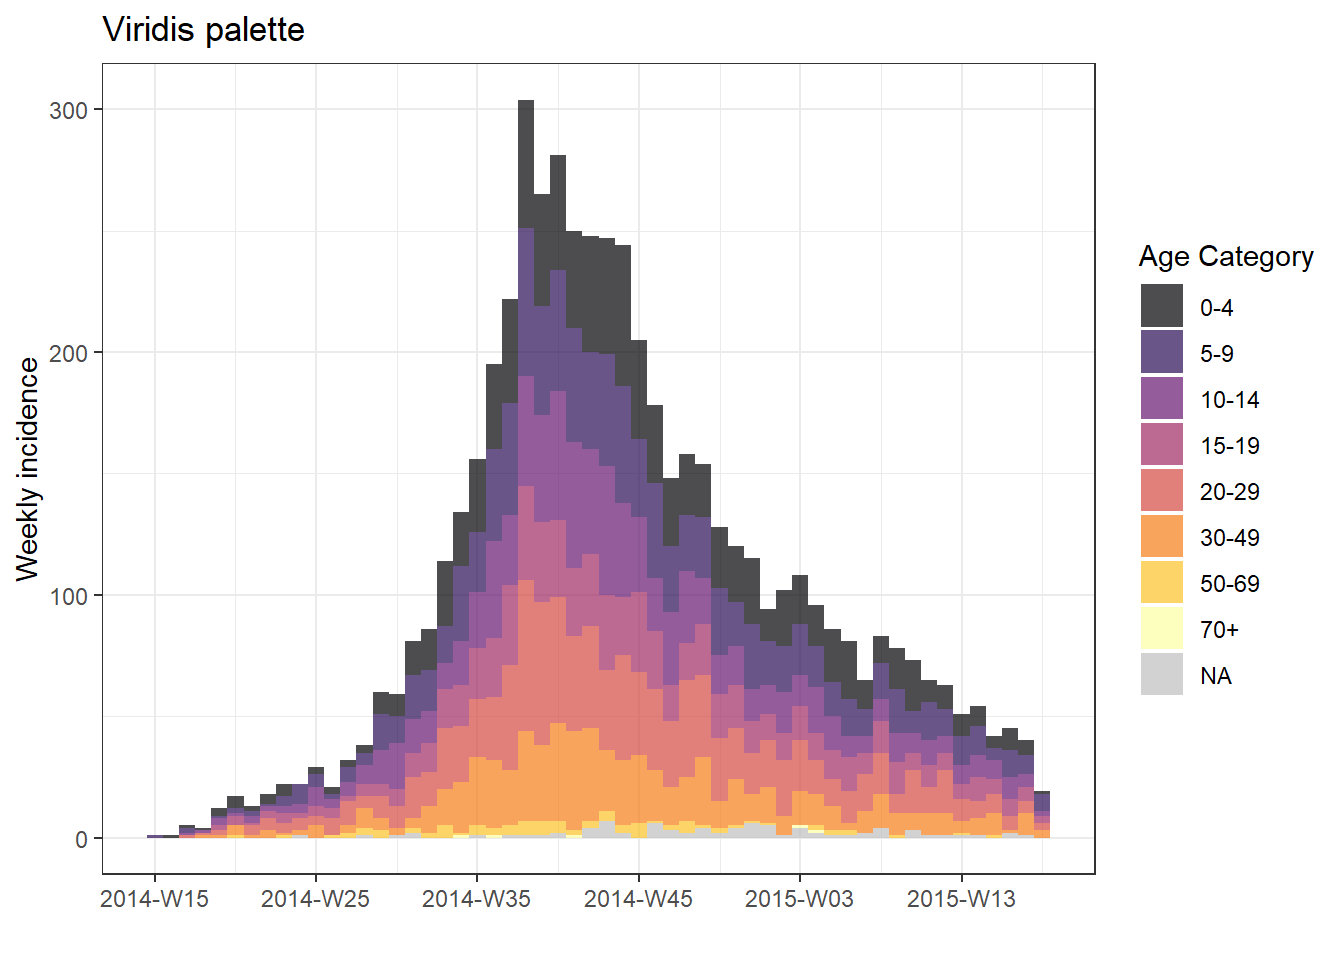
\includegraphics{C:/Users/Neale/ONEDRI~1/DOCUME~1/ANALYT~1/R/Projects/RHANDB~1/EPI_R_~1/pages_OUTPU~1/AGE_PY~1/figure-latex/unnamed-chunk-28-1.pdf}

\hypertarget{likert-scale}{%
\subsection{Likert Scale}\label{likert-scale}}

The techniques used to make a population pyramid with \texttt{ggplot()}
can also be used to make plots of Likert-scale survey data.

Import the data

\begin{Shaded}
\begin{Highlighting}[]
\CommentTok{\# import the likert survey response data}
\NormalTok{likert\_data \textless{}{-}}\StringTok{ }\NormalTok{rio}\OperatorTok{::}\KeywordTok{import}\NormalTok{(}\StringTok{"likert\_data.csv"}\NormalTok{)}
\end{Highlighting}
\end{Shaded}

Start with data that looks like this, with a categorical classification
of each respondent (\texttt{status}) and their answers to 8 questions on
a 4-point Likert-type scale (``Very poor'', ``Poor'', ``Good'', ``Very
good'').

\begin{Shaded}
\begin{Highlighting}[]
\CommentTok{\# display the linelist data as a table}
\NormalTok{DT}\OperatorTok{::}\KeywordTok{datatable}\NormalTok{(likert\_data, }\DataTypeTok{rownames =} \OtherTok{FALSE}\NormalTok{, }\DataTypeTok{filter=}\StringTok{"top"}\NormalTok{, }\DataTypeTok{options =} \KeywordTok{list}\NormalTok{(}\DataTypeTok{pageLength =} \DecValTok{10}\NormalTok{, }\DataTypeTok{scrollX=}\NormalTok{T) )}
\end{Highlighting}
\end{Shaded}

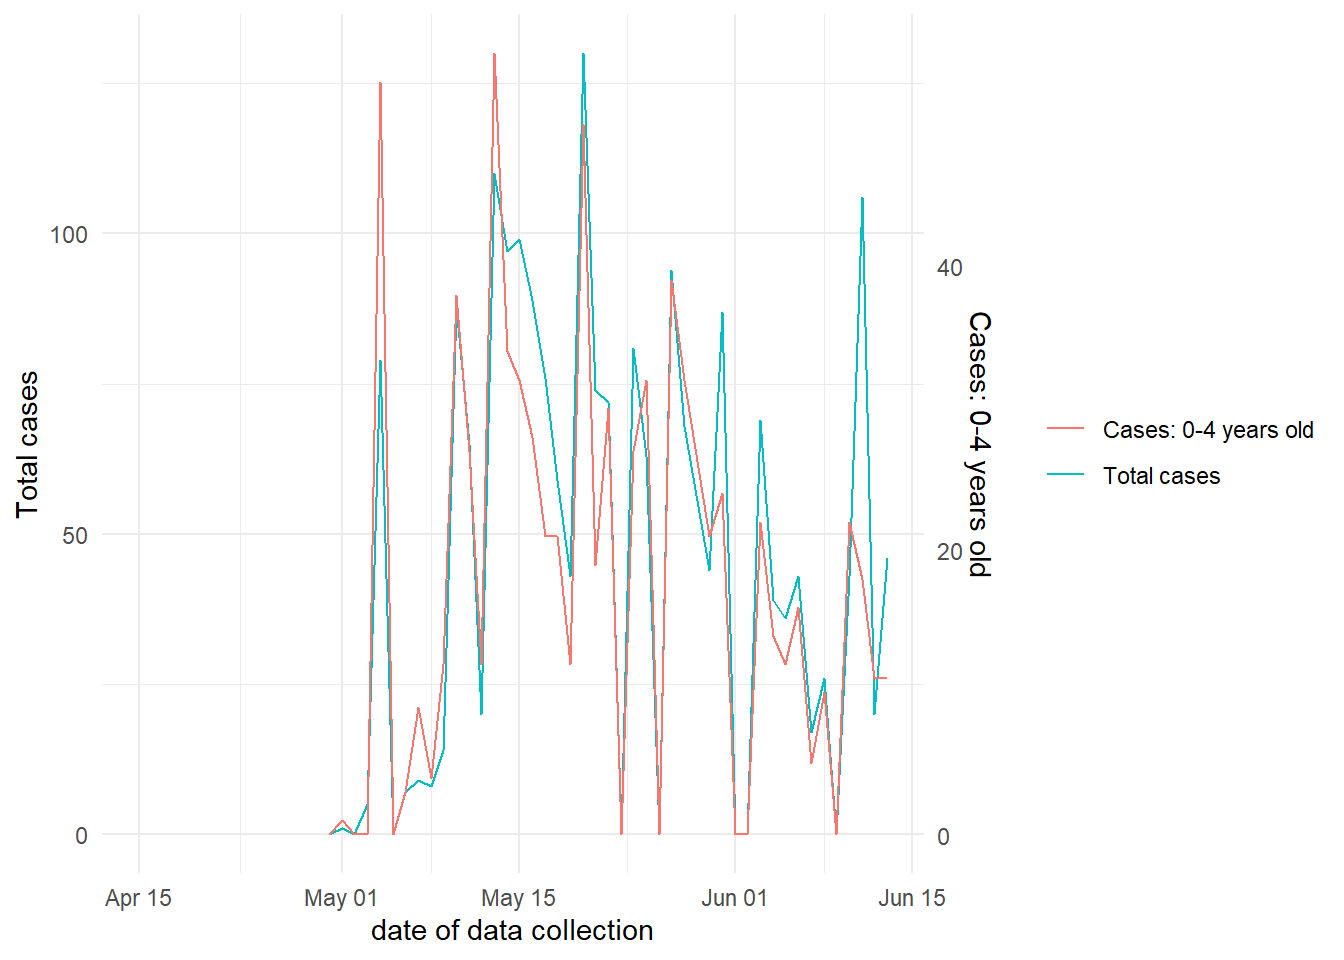
\includegraphics{C:/Users/Neale/ONEDRI~1/DOCUME~1/ANALYT~1/R/Projects/RHANDB~1/EPI_R_~1/pages_OUTPU~1/AGE_PY~1/figure-latex/unnamed-chunk-32-1.pdf}

First, some data management steps:

\begin{itemize}
\tightlist
\item
  Pivot the data longer\\
\item
  Create new column \texttt{direction} depending on whether response was
  generally ``positive'' or ``negative''\\
\item
  Set the Factor level order for the \texttt{status} column and the
  \texttt{Response} column\\
\item
  Store the max count value so limits of plot are appropriate
\end{itemize}

\begin{Shaded}
\begin{Highlighting}[]
\NormalTok{melted \textless{}{-}}\StringTok{ }\KeywordTok{pivot\_longer}\NormalTok{(likert\_data, Q1}\OperatorTok{:}\NormalTok{Q8, }\DataTypeTok{names\_to =} \StringTok{"Question"}\NormalTok{, }\DataTypeTok{values\_to =} \StringTok{"Response"}\NormalTok{) }\OperatorTok{\%\textgreater{}\%}\StringTok{ }
\StringTok{     }\KeywordTok{mutate}\NormalTok{(}\DataTypeTok{direction =} \KeywordTok{case\_when}\NormalTok{(}
\NormalTok{               Response }\OperatorTok{\%in\%}\StringTok{ }\KeywordTok{c}\NormalTok{(}\StringTok{"Poor"}\NormalTok{,}\StringTok{"Very Poor"}\NormalTok{) }\OperatorTok{\textasciitilde{}}\StringTok{ "Negative"}\NormalTok{,}
\NormalTok{               Response }\OperatorTok{\%in\%}\StringTok{ }\KeywordTok{c}\NormalTok{(}\StringTok{"Good"}\NormalTok{, }\StringTok{"Very Good"}\NormalTok{) }\OperatorTok{\textasciitilde{}}\StringTok{ "Positive"}\NormalTok{,}
               \OtherTok{TRUE} \OperatorTok{\textasciitilde{}}\StringTok{ "Unknown"}\NormalTok{),}
            \DataTypeTok{status =} \KeywordTok{factor}\NormalTok{(status, }\DataTypeTok{levels =} \KeywordTok{rev}\NormalTok{(}\KeywordTok{c}\NormalTok{(}
                 \StringTok{"Senior"}\NormalTok{, }\StringTok{"Intermediate"}\NormalTok{, }\StringTok{"Junior"}\NormalTok{))),}
            \DataTypeTok{Response =} \KeywordTok{factor}\NormalTok{(Response, }\DataTypeTok{levels =} \KeywordTok{c}\NormalTok{(}\StringTok{"Very Good"}\NormalTok{, }\StringTok{"Good"}\NormalTok{,}
                                             \StringTok{"Very Poor"}\NormalTok{, }\StringTok{"Poor"}\NormalTok{))) }\CommentTok{\# must reverse Very Poor and Poor for ordering to work}

\NormalTok{melted\_max \textless{}{-}}\StringTok{ }\NormalTok{melted }\OperatorTok{\%\textgreater{}\%}\StringTok{ }
\StringTok{   }\KeywordTok{group\_by}\NormalTok{(status, Question) }\OperatorTok{\%\textgreater{}\%}\StringTok{ }
\StringTok{   }\KeywordTok{summarize}\NormalTok{(}\DataTypeTok{n =} \KeywordTok{n}\NormalTok{())}

\NormalTok{melted\_max \textless{}{-}}\StringTok{ }\KeywordTok{max}\NormalTok{(melted\_max}\OperatorTok{$}\NormalTok{n, }\DataTypeTok{na.rm=}\NormalTok{T)}
\end{Highlighting}
\end{Shaded}

Now make the plot:

\begin{Shaded}
\begin{Highlighting}[]
\CommentTok{\# make plot}
\KeywordTok{ggplot}\NormalTok{()}\OperatorTok{+}
\StringTok{     }\CommentTok{\# bar graph of the "negative" responses }
\StringTok{     }\KeywordTok{geom\_bar}\NormalTok{(}\DataTypeTok{data =} \KeywordTok{filter}\NormalTok{(melted,}
\NormalTok{                            direction }\OperatorTok{==}\StringTok{ "Negative"}\NormalTok{), }
              \KeywordTok{aes}\NormalTok{(}\DataTypeTok{x =}\NormalTok{ status,}
                        \DataTypeTok{y=}\NormalTok{..count..}\OperatorTok{*}\NormalTok{(}\OperatorTok{{-}}\DecValTok{1}\NormalTok{),    }\CommentTok{\# counts inverted to negative}
                        \DataTypeTok{fill =}\NormalTok{ Response),}
                    \DataTypeTok{color =} \StringTok{"black"}\NormalTok{,}
                    \DataTypeTok{closed =} \StringTok{"left"}\NormalTok{, }
                    \DataTypeTok{position =} \StringTok{"stack"}\NormalTok{)}\OperatorTok{+}
\StringTok{     }
\StringTok{     }\CommentTok{\# bar graph of the "positive responses}
\StringTok{     }\KeywordTok{geom\_bar}\NormalTok{(}\DataTypeTok{data =} \KeywordTok{filter}\NormalTok{(melted, direction }\OperatorTok{==}\StringTok{ "Positive"}\NormalTok{),}
              \KeywordTok{aes}\NormalTok{(}\DataTypeTok{x =}\NormalTok{ status, }\DataTypeTok{fill =}\NormalTok{ Response),}
              \DataTypeTok{colour =} \StringTok{"black"}\NormalTok{,}
              \DataTypeTok{closed =} \StringTok{"left"}\NormalTok{,}
              \DataTypeTok{position =} \StringTok{"stack"}\NormalTok{)}\OperatorTok{+}
\StringTok{     }
\StringTok{     }\CommentTok{\# flip the X and Y axes}
\StringTok{     }\KeywordTok{coord\_flip}\NormalTok{()}\OperatorTok{+}
\StringTok{  }
\StringTok{     }\CommentTok{\# Black vertical line at 0}
\StringTok{     }\KeywordTok{geom\_hline}\NormalTok{(}\DataTypeTok{yintercept =} \DecValTok{0}\NormalTok{, }\DataTypeTok{color =} \StringTok{"black"}\NormalTok{, }\DataTypeTok{size=}\DecValTok{1}\NormalTok{)}\OperatorTok{+}
\StringTok{     }
\StringTok{    }\CommentTok{\# convert labels to all positive numbers}
\StringTok{    }\KeywordTok{scale\_y\_continuous}\NormalTok{(}\DataTypeTok{limits =} \KeywordTok{c}\NormalTok{(}\OperatorTok{{-}}\KeywordTok{ceiling}\NormalTok{(melted\_max}\OperatorTok{/}\DecValTok{10}\NormalTok{)}\OperatorTok{*}\DecValTok{11}\NormalTok{, }\KeywordTok{ceiling}\NormalTok{(melted\_max}\OperatorTok{/}\DecValTok{10}\NormalTok{)}\OperatorTok{*}\DecValTok{10}\NormalTok{),   }\CommentTok{\# seq from neg to pos by 10, edges rounded outward to nearest 5}
                       \DataTypeTok{breaks =} \KeywordTok{seq}\NormalTok{(}\OperatorTok{{-}}\KeywordTok{ceiling}\NormalTok{(melted\_max}\OperatorTok{/}\DecValTok{10}\NormalTok{)}\OperatorTok{*}\DecValTok{10}\NormalTok{, }\KeywordTok{ceiling}\NormalTok{(melted\_max}\OperatorTok{/}\DecValTok{10}\NormalTok{)}\OperatorTok{*}\DecValTok{10}\NormalTok{, }\DecValTok{10}\NormalTok{),}
                       \DataTypeTok{labels =} \KeywordTok{abs}\NormalTok{(}\KeywordTok{unique}\NormalTok{(}\KeywordTok{c}\NormalTok{(}\KeywordTok{seq}\NormalTok{(}\OperatorTok{{-}}\KeywordTok{ceiling}\NormalTok{(melted\_max}\OperatorTok{/}\DecValTok{10}\NormalTok{)}\OperatorTok{*}\DecValTok{10}\NormalTok{, }\DecValTok{0}\NormalTok{, }\DecValTok{10}\NormalTok{),}
                                            \KeywordTok{seq}\NormalTok{(}\DecValTok{0}\NormalTok{, }\KeywordTok{ceiling}\NormalTok{(melted\_max}\OperatorTok{/}\DecValTok{10}\NormalTok{)}\OperatorTok{*}\DecValTok{10}\NormalTok{, }\DecValTok{10}\NormalTok{))))) }\OperatorTok{+}
\StringTok{     }
\StringTok{    }\CommentTok{\# color scales manually assigned }
\StringTok{    }\KeywordTok{scale\_fill\_manual}\NormalTok{(}\DataTypeTok{values =} \KeywordTok{c}\NormalTok{(}\StringTok{"Very Good"}\NormalTok{  =}\StringTok{ "green4"}\NormalTok{, }\CommentTok{\# assigns colors}
                                  \StringTok{"Good"}\NormalTok{      =}\StringTok{ "green3"}\NormalTok{,}
                                  \StringTok{"Poor"}\NormalTok{      =}\StringTok{ "yellow"}\NormalTok{,}
                                  \StringTok{"Very Poor"}\NormalTok{ =}\StringTok{ "red3"}\NormalTok{),}
                       \DataTypeTok{breaks =} \KeywordTok{c}\NormalTok{(}\StringTok{"Very Good"}\NormalTok{, }\StringTok{"Good"}\NormalTok{, }\StringTok{"Poor"}\NormalTok{, }\StringTok{"Very Poor"}\NormalTok{))}\OperatorTok{+}\StringTok{ }\CommentTok{\# orders the legend}
\StringTok{     }
\StringTok{    }
\StringTok{     }
\StringTok{    }\CommentTok{\# facet the entire plot so each question is a sub{-}plot}
\StringTok{    }\KeywordTok{facet\_wrap}\NormalTok{(}\OperatorTok{\textasciitilde{}}\NormalTok{Question, }\DataTypeTok{ncol =} \DecValTok{3}\NormalTok{)}\OperatorTok{+}
\StringTok{     }
\StringTok{    }\CommentTok{\# labels, titles, caption}
\StringTok{    }\KeywordTok{labs}\NormalTok{(}\DataTypeTok{x =} \StringTok{"Respondent status"}\NormalTok{,}
          \DataTypeTok{y =} \StringTok{"Number of responses"}\NormalTok{,}
          \DataTypeTok{fill =} \StringTok{""}\NormalTok{)}\OperatorTok{+}
\StringTok{     }\KeywordTok{ggtitle}\NormalTok{(}\KeywordTok{str\_glue}\NormalTok{(}\StringTok{"Likert{-}style responses}\CharTok{\textbackslash{}n}\StringTok{n = \{nrow(likert\_data)\}"}\NormalTok{))}\OperatorTok{+}

\StringTok{     }\CommentTok{\# aesthetic settings}
\StringTok{     }\KeywordTok{theme\_minimal}\NormalTok{()}\OperatorTok{+}
\StringTok{     }\KeywordTok{theme}\NormalTok{(}\DataTypeTok{axis.text =} \KeywordTok{element\_text}\NormalTok{(}\DataTypeTok{size =} \DecValTok{12}\NormalTok{),}
           \DataTypeTok{axis.title =} \KeywordTok{element\_text}\NormalTok{(}\DataTypeTok{size =} \DecValTok{14}\NormalTok{, }\DataTypeTok{face =} \StringTok{"bold"}\NormalTok{),}
           \DataTypeTok{strip.text =} \KeywordTok{element\_text}\NormalTok{(}\DataTypeTok{size =} \DecValTok{14}\NormalTok{, }\DataTypeTok{face =} \StringTok{"bold"}\NormalTok{),  }\CommentTok{\# facet sub{-}titles}
           \DataTypeTok{plot.title =} \KeywordTok{element\_text}\NormalTok{(}\DataTypeTok{size =} \DecValTok{20}\NormalTok{, }\DataTypeTok{face =} \StringTok{"bold"}\NormalTok{),}
           \DataTypeTok{panel.background =} \KeywordTok{element\_rect}\NormalTok{(}\DataTypeTok{fill =} \OtherTok{NA}\NormalTok{, }\DataTypeTok{color =} \StringTok{"black"}\NormalTok{)) }\CommentTok{\# black box around each facet}
\end{Highlighting}
\end{Shaded}

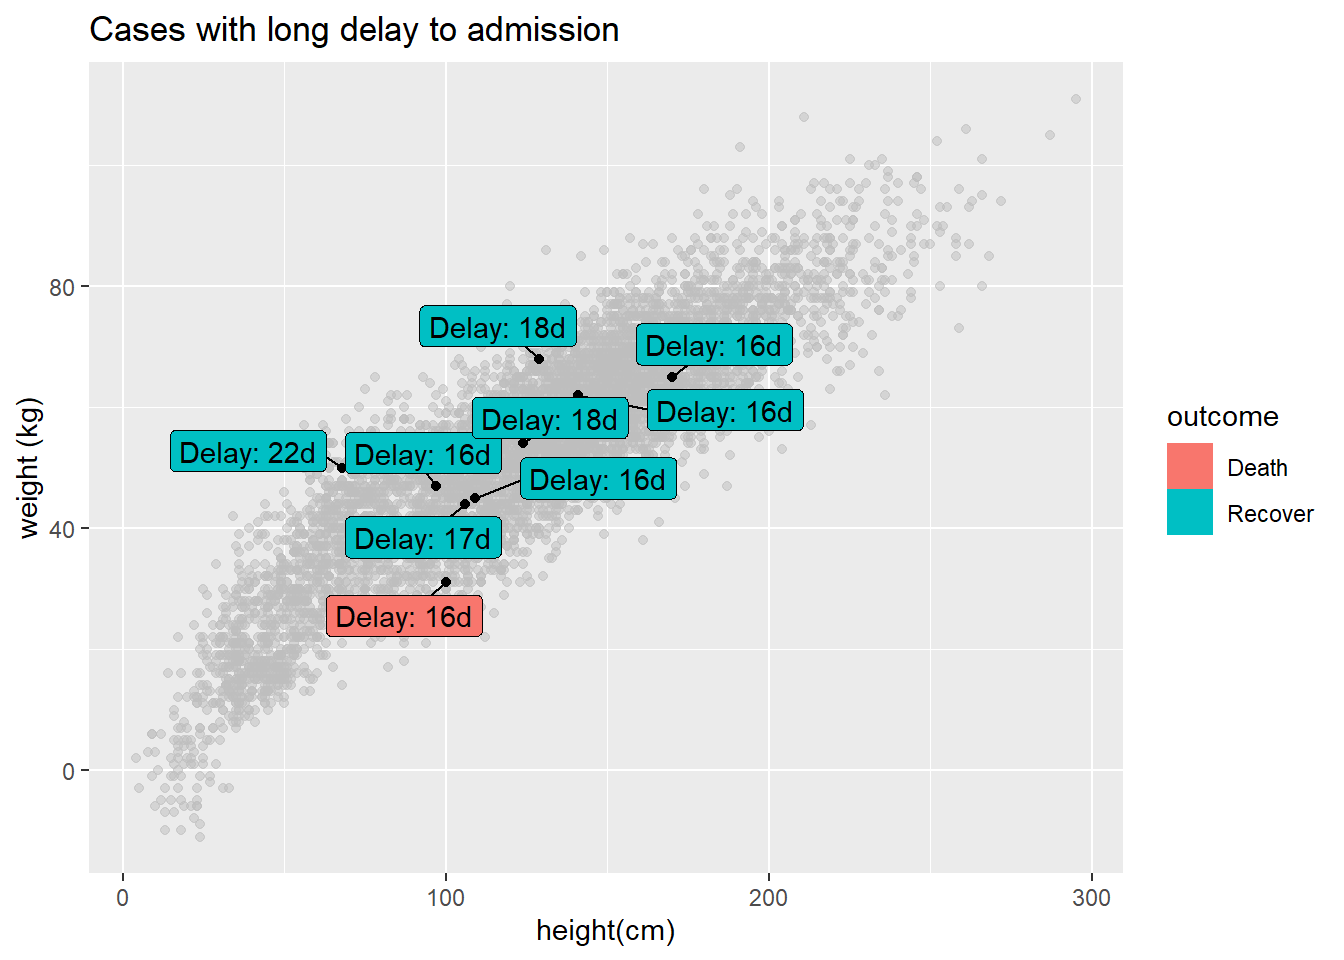
\includegraphics{C:/Users/Neale/ONEDRI~1/DOCUME~1/ANALYT~1/R/Projects/RHANDB~1/EPI_R_~1/pages_OUTPU~1/AGE_PY~1/figure-latex/unnamed-chunk-34-1.pdf}

\hypertarget{resources}{%
\subsection{Resources}\label{resources}}

This tab should stay with the name ``Resources''. Links to other online
tutorials or resources.

\end{document}
